\chapter{Properties of robot}
\section{Planar robot with 2 degrees of freedom}
The first task is to derive the equation of motion for a 2 \ac{DOF} planar robot using Lagrange formalism. The schematic of such a robot is shown in Figure \ref{fig:planar_robot_schematic}. This robot consists of two drives, connected by links which have the mass at the tip of them.
\begin{figure}[H]
	\centering
	\newcommand{\nvar}[2]{%
	\newlength{#1}
	\setlength{#1}{#2}
}

% Define a few constants for drawing
\nvar{\dg}{0.3cm}
\def\dw{0.25}\def\dh{0.5}
\nvar{\ddx}{1.5cm}

% Define commands for links, joints and such
\def\link{\draw [double distance=1.5mm, very thick] (0,0)--}
\def\joint{%
	\filldraw [fill=white] (0,0) circle (5pt);
	\fill[black] circle (2pt);
}
\def\grip{%
	\draw[ultra thick](0cm,\dg)--(0cm,-\dg);
	\fill (0cm, 0.5\dg)+(0cm,1.5pt) -- +(0.6\dg,0cm) -- +(0pt,-1.5pt);
	\fill (0cm, -0.5\dg)+(0cm,1.5pt) -- +(0.6\dg,0cm) -- +(0pt,-1.5pt);
}
\def\robotbase{%
	\draw[rounded corners=8pt] (-\dw,-\dh)-- (-\dw, 0) --
	(0,\dh)--(\dw,0)--(\dw,-\dh);
	\draw (-0.5,-\dh)-- (0.5,-\dh);
	\fill[pattern=north east lines] (-0.5,-1) rectangle (0.5,-\dh);
}

% Draw an angle annotation
% Input:
%   #1 Angle
%   #2 Label
% Example:
%   \angann{30}{$\theta_1$}
\newcommand{\angann}[2]{%
	\begin{scope}[]
		\draw [dashed] (0,0) -- (1.2\ddx,0pt);
		\draw [->, shorten >=3.5pt] (\ddx,0pt) arc (0:#1:\ddx);
		% Unfortunately automatic node placement on an arc is not supported yet.
		% We therefore have to compute an appropriate coordinate ourselves.
		\node at (#1/2-2:\ddx+8pt) {#2};
	\end{scope}
}

% Draw line annotation
% Input:
%   #1 Line offset (optional)
%   #2 Line angle
%   #3 Line length
%   #5 Line label
% Example:
%   \lineann[1]{30}{2}{$L_1$}
\newcommand{\lineann}[4][0.5]{%
	\begin{scope}[rotate=#2,inner sep=2pt]
		\draw[dashed] (0,0) -- +(0,#1)
		node [coordinate, near end] (a) {};
		\draw[dashed] (#3,0) -- +(0,#1)
		node [coordinate, near end] (b) {};
		\draw[|<->|] (a) -- node[fill=white] {#4} (b);
	\end{scope}
}

% Define the kinematic parameters of the three link manipulator.
\def\thetaone{30}
\def\Lone{2}
\def\thetatwo{30}
\def\Ltwo{2}

\begin{tikzpicture}[scale=1.5]
\robotbase
\angann{\thetaone}{$\theta_1$}
\lineann[0.7]{\thetaone}{\Lone}{$a_1$}
\link(\thetaone:\Lone);
\joint
\draw [<->,thick] (0,3) node (yaxis) [above] {$y$}
|- (3,0) node (xaxis) [right] {$x$};
\begin{scope}[shift=(\thetaone:\Lone), rotate=\thetaone]
\node [yshift = -0.5cm, xshift=0.2cm] () {$m_1$};
\angann{\thetatwo}{$\theta_2$}
\lineann[-1.5]{\thetatwo}{\Ltwo}{$a_2$}
\link(\thetatwo:\Ltwo);
\joint
\begin{scope}[shift=(\thetatwo:\Ltwo), rotate=\thetatwo]
\joint
\node [yshift=.4cm] {$m_2$};
\end{scope}
\end{scope}
\end{tikzpicture}
	\caption{Schematic of a planar robot with 2 degrees of freedom}
	\label{fig:planar_robot_schematic}
\end{figure}
The generalised coordinates of the system are the angles $\theta_1$ and $\theta_2$, afterwards denoted by $q_1$ and $q_2$ respectively. As the masses are assumed to be point masses, the according position vectors can be used to derive the kinetic and the potential energy. The position and velocity vectors are given by:
\begin{align*}
	\mathbf{r}_1 = \left(\begin{array}{c}
	a_1\cos(q_1)\\
	a_1\sin(q_1)
	\end{array}\right) && \mathbf{r}_2 = \left(\begin{array}{c}
	a_1\cos(q_1) + a_2\cos(q_1+q_2)\\
	a_1\sin(q_1) + a_2\sin(q_1+q_2)
	\end{array}\right)\\
	\dot{\mathbf{r}}_1 = \left(\begin{array}{c}
	-a_1\sin(q_1)\dot{q}_1\\
	a_1\cos(q_1)\dot{q}_1
	\end{array}\right) && \dot{\mathbf{r}}_2 = \left(\begin{array}{c}
	-a_1\sin(q_1)\dot{q}_1 - a_2\sin(q_1+q_2)(\dot{q}_1 + \dot{q}_2)\\
	a_1\cos(q_1)\dot{q}_1 + a_2\cos(q_1+q_2)(\dot{q}_1 + \dot{q}_2)
	\end{array}\right)
\end{align*}
The kinetic energy $T$ of the robot arm is described by the following equation:
\begin{align}
	T =& \frac{m_1}{2}\dot{\mathbf{r}}_1^T\dot{\mathbf{r}}_1 + \frac{m_2}{2}\dot{\mathbf{r}}_2^T\dot{\mathbf{r}}_2\nonumber\\
	=& \frac{a_1^2 (m_1 + m_2) + a_2^2 m_2}{2} \dot{q}_1^2 + \frac{a_2^2 m_2}{2} \dot{q}_2 + a_2m_2(a_2\dot{q}_2 + a_1\cos(q_2)\dot{q}_1 + a_1\cos(q_2)\dot{q}_2)\dot{q}_1
	\label{eq:ch1_kinetic}
\end{align}
The potential energy $V$ is given by:
\begin{equation}
	V = m_1 g y_1 + m_2 g y_2 = a_1 m_1 g \sin(q_1) + m_2 g (a_1 \sin(q_1) + a_2 \sin (q_1 + q_2))
	\label{eq:ch1_potential}
\end{equation}
The Lagrangian $L$, which is needed for the Lagrange formalism, is defined as the difference of the kinetic energy $T$ and the potential energy $V$:
\begin{equation}
	L = T - V
	\label{eq:ch1_lagrangian}
\end{equation}
\newpage
The Lagrange formalism is given by the following equation:
\begin{gather}
	\frac{d}{dt}\left(\frac{\partial L}{\partial \dot{q}_k}\right) - \frac{\partial L}{\partial q_k} = Q_k
	\label{eq:ch1_lagform}
	\intertext{where:}
	\begin{tabular}{>{$}l<{$} @{${}:{}$} l}
	q_k & k\textsuperscript{th} generalised coordinate\\
	\dot{q}_k & k\textsuperscript{th} generalised velocity\\
	Q_k & k\textsuperscript{th} generalised force
	\end{tabular}\nonumber
\end{gather}
Inserting Equations \ref{eq:ch1_kinetic} and \ref{eq:ch1_potential} into \ref{eq:ch1_lagrangian} and applying the result on \ref{eq:ch1_lagform}, results in the differential equations, which describe the movement of the planar robot. The resulting system description has the following form:
\begin{gather}
\mathbf{\tau} = \mathbf{M}(\mathbf{q})\mathbf{\ddot{q}} + \mathbf{v}(\mathbf{q}, \mathbf{\dot{q}}) + \mathbf{g}(\mathbf{q}) + \mathbf{\tau}_D
\label{eq:ch1_robotdynamics}
\intertext{where:}
\begin{tabular}{>{$}l<{$} @{${}={}$} l}
	\mathbf{\tau} & input torque vector \\
	\mathbf{M}(\mathbf{q}) & inertia matrix\\
	\mathbf{v}(\mathbf{q}, \mathbf{\dot{q}}) & centrifugal/corriolis vector\\
	\mathbf{g}(\mathbf{q}) & gravitation vector\\
	\mathbf{\tau}_D & disturbance vector
\end{tabular}\nonumber
\end{gather}
Often, the term $\mathbf{v}(\mathbf{q}, \mathbf{\dot{q}}) + \mathbf{g}(\mathbf{q})$ is gathered and denoted by $\mathbf{n}(\mathbf{q}, \mathbf{\dot{q}})$. The result of the calculation is given by:
\begin{align*}
	\tau &= \left(\begin{array}{cc} {a_1}^2 m_1 + {a_1}^2 m_2 + {a_2}^2 m_2 + 2 a_1 a_2 m_2 \cos\!\left(q_2\right) & a_2 m_2 \left(a_2 + a_1 \cos\!\left(q_2\right)\right)\\ a_2 m_2 \left(a_2 + a_1 \cos\!\left(q_2\right)\right) & {a_2}^2 m_2 \end{array}\right)
\left(\begin{array}{c}
	\ddot{q}_1\\ \ddot{q}_2
	\end{array}\right) \\
	 &+ \left(\begin{array}{c} - a_1 a_2 m_2 \dot{q}_{2} \sin\!\left(q_2\right) \left(2 \dot{q}_{1} + \dot{q}_{2}\right)\\ a_1 a_2 m_2 {\dot{q}_{1}}^2 \sin\!\left(q_2\right) \end{array}\right)
\\
	 &+ \left(\begin{array}{c} g m_2 \left(a_2 \cos\!\left(q_1 + q_2\right) + a_1 \cos\!\left(q_1\right)\right) + a_1 g m_1 \cos\!\left(q_1\right)\\ a_2 g m_2 \cos\!\left(q_1 + q_2\right) \end{array}\right)

\end{align*}
In this result the disturbance vector $\tau_D$ was set to zero, because it is unknown.\\
As a next step, the direct kinematics and the Jacobian matrix have to be found. The direct kinematic was already calculated in the beginning and is denoted by $\mathbf{r}_2$:
\begin{equation*}
	\mathbf{r}_2 = \left(\begin{array}{c}
	a_1\cos(q_1) + a_2\cos(q_1+q_2)\\
	a_1\sin(q_1) + a_2\sin(q_1+q_2)
	\end{array}\right)
\end{equation*}
The Jacobian is the partial derivative of the position vector with respect to the generalised coordinates:
\begin{equation*}
	\mathbf{J}(\mathbf{q}) = \frac{\partial \mathbf{r}_2}{\partial \mathbf{q}} = \left(\begin{array}{cc}  - a_2 \sin\!\left(q_1 + q_2\right) - a_1 \sin\!\left(q_1\right) & - a_2 \sin\!\left(q_1 + q_2\right)\\ a_2 \cos\!\left(q_1 + q_2\right) + a_1 \cos\!\left(q_1\right) & a_2 \cos\!\left(q_1 + q_2\right) \end{array}\right)

\end{equation*}
For all further considerations, the following state vector is introduced:
\begin{equation*}
	\mathbf{x}=\left(\begin{array}{c}
q_1\\ q_2 \\ \dot{q}_1 \\ \dot{q}_2
\end{array}\right)
\end{equation*}
The next step is to check the plausibility of the equations of motion by simulation.
\section{Simulation of robot dynamics}
To check, if the previously derived dynamic equations are plausible, some simulations are done. For these simulations, the following values are used for the parameters:
\begin{align*}
	m_1 = m_2 &= 1\,\mathrm{kg}\\
	a_1 = a_2 &= 1\,\mathrm{m}\\
	g &= 9.81\,\mathrm{\frac{m}{s^2}}
\end{align*}As a first simulation, the stable, downright equilibrium point is used as initial condition. The expected result is, that no movement occurs, as the system always stays in its equilibrium. For the next simulation, the unstable, upper equilibrium is used. Again, no movement is to be expected, as the initial condition is again an equilibrium point and no external force is applied. As a last simulation, an initial condition of $\mathbf{x}_0 =\left( \begin{array}{cccc}
	0 & 0 & 0 & 0
\end{array}\right)^T$ is used. The expected result is some kind of chaotic oscillation of both joints.\\
Figure \ref{fig:ch1_model1} shows the results of the simulation with the stable equilibrium point as initial condition. As expected, the position remains zero for the whole simulation. The small values of the velocities, somewhere around $10^{-14}$, are caused by numerical errors.
\begin{figure}[H]
	\centering
	% This file was created by matlab2tikz v0.4.3.
% Copyright (c) 2008--2013, Nico Schlömer <nico.schloemer@gmail.com>
% All rights reserved.
% 
% The latest updates can be retrieved from
%   http://www.mathworks.com/matlabcentral/fileexchange/22022-matlab2tikz
% where you can also make suggestions and rate matlab2tikz.
% 
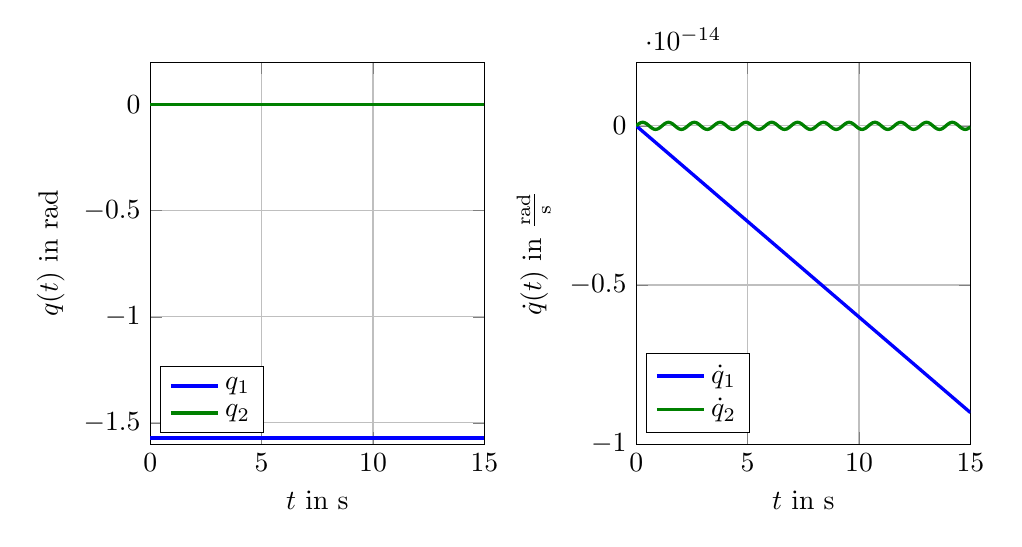
\begin{tikzpicture}

\begin{axis}[%
width=0.35\textwidth,
height=0.4\textwidth,
scale only axis,
xmin=0,
xmax=15,
xlabel={$t$ in $\mathrm{s}$},
xmajorgrids,
ymin=-1.6,
ymax=0.2,
ylabel={$q(t)$ in $\mathrm{rad}$},
ymajorgrids,
name=plot1,
legend style={at={(0.03,0.03)},anchor=south west,draw=black,fill=white,legend cell align=left}
]
\addplot [
color=blue,
solid,
line width=1.2pt
]
table[row sep=crcr]{
0 -1.5707963267949\\
0.05 -1.5707963267949\\
0.1 -1.5707963267949\\
0.15 -1.5707963267949\\
0.2 -1.5707963267949\\
0.25 -1.5707963267949\\
0.3 -1.5707963267949\\
0.35 -1.5707963267949\\
0.4 -1.5707963267949\\
0.45 -1.5707963267949\\
0.5 -1.5707963267949\\
0.55 -1.5707963267949\\
0.6 -1.5707963267949\\
0.65 -1.5707963267949\\
0.700000000000001 -1.5707963267949\\
0.750000000000001 -1.5707963267949\\
0.800000000000001 -1.5707963267949\\
0.850000000000001 -1.5707963267949\\
0.900000000000001 -1.5707963267949\\
0.950000000000001 -1.5707963267949\\
1 -1.5707963267949\\
1.05 -1.5707963267949\\
1.09999999999999 -1.5707963267949\\
1.14999999999998 -1.5707963267949\\
1.19999999999998 -1.5707963267949\\
1.24999999999997 -1.5707963267949\\
1.29999999999997 -1.5707963267949\\
1.34999999999996 -1.5707963267949\\
1.39999999999996 -1.5707963267949\\
1.44999999999995 -1.5707963267949\\
1.49999999999995 -1.5707963267949\\
1.54999999999994 -1.5707963267949\\
1.59999999999993 -1.5707963267949\\
1.64999999999993 -1.5707963267949\\
1.69999999999992 -1.5707963267949\\
1.74999999999992 -1.5707963267949\\
1.79999999999991 -1.5707963267949\\
1.84999999999991 -1.5707963267949\\
1.8999999999999 -1.5707963267949\\
1.9499999999999 -1.5707963267949\\
1.99999999999989 -1.5707963267949\\
2.04999999999989 -1.5707963267949\\
2.09999999999988 -1.5707963267949\\
2.14999999999987 -1.5707963267949\\
2.19999999999987 -1.5707963267949\\
2.24999999999986 -1.5707963267949\\
2.29999999999986 -1.5707963267949\\
2.34999999999985 -1.5707963267949\\
2.39999999999985 -1.5707963267949\\
2.44999999999984 -1.5707963267949\\
2.49999999999984 -1.5707963267949\\
2.54999999999983 -1.5707963267949\\
2.59999999999982 -1.5707963267949\\
2.64999999999982 -1.5707963267949\\
2.69999999999981 -1.5707963267949\\
2.74999999999981 -1.5707963267949\\
2.7999999999998 -1.5707963267949\\
2.8499999999998 -1.5707963267949\\
2.89999999999979 -1.5707963267949\\
2.94999999999979 -1.5707963267949\\
2.99999999999978 -1.5707963267949\\
3.04999999999978 -1.5707963267949\\
3.09999999999977 -1.5707963267949\\
3.14999999999976 -1.5707963267949\\
3.19999999999976 -1.5707963267949\\
3.24999999999975 -1.5707963267949\\
3.29999999999975 -1.5707963267949\\
3.34999999999974 -1.5707963267949\\
3.39999999999974 -1.5707963267949\\
3.44999999999973 -1.5707963267949\\
3.49999999999973 -1.5707963267949\\
3.54999999999972 -1.5707963267949\\
3.59999999999971 -1.5707963267949\\
3.64999999999971 -1.5707963267949\\
3.6999999999997 -1.5707963267949\\
3.7499999999997 -1.5707963267949\\
3.79999999999969 -1.5707963267949\\
3.84999999999969 -1.5707963267949\\
3.89999999999968 -1.5707963267949\\
3.94999999999968 -1.5707963267949\\
3.99999999999967 -1.5707963267949\\
4.04999999999969 -1.5707963267949\\
4.0999999999997 -1.5707963267949\\
4.14999999999972 -1.5707963267949\\
4.19999999999974 -1.5707963267949\\
4.24999999999975 -1.5707963267949\\
4.29999999999977 -1.5707963267949\\
4.34999999999979 -1.5707963267949\\
4.3999999999998 -1.5707963267949\\
4.44999999999982 -1.5707963267949\\
4.49999999999984 -1.5707963267949\\
4.54999999999985 -1.5707963267949\\
4.59999999999987 -1.5707963267949\\
4.64999999999989 -1.5707963267949\\
4.6999999999999 -1.5707963267949\\
4.74999999999992 -1.5707963267949\\
4.79999999999994 -1.5707963267949\\
4.84999999999995 -1.5707963267949\\
4.89999999999997 -1.5707963267949\\
4.94999999999999 -1.5707963267949\\
5 -1.5707963267949\\
5.05000000000002 -1.5707963267949\\
5.10000000000004 -1.5707963267949\\
5.15000000000005 -1.5707963267949\\
5.20000000000007 -1.5707963267949\\
5.25000000000009 -1.5707963267949\\
5.3000000000001 -1.5707963267949\\
5.35000000000012 -1.5707963267949\\
5.40000000000014 -1.5707963267949\\
5.45000000000015 -1.5707963267949\\
5.50000000000017 -1.5707963267949\\
5.55000000000019 -1.5707963267949\\
5.6000000000002 -1.5707963267949\\
5.65000000000022 -1.5707963267949\\
5.70000000000024 -1.5707963267949\\
5.75000000000025 -1.5707963267949\\
5.80000000000027 -1.5707963267949\\
5.85000000000029 -1.5707963267949\\
5.90000000000031 -1.5707963267949\\
5.95000000000032 -1.5707963267949\\
6.00000000000034 -1.5707963267949\\
6.05000000000036 -1.5707963267949\\
6.10000000000037 -1.5707963267949\\
6.15000000000039 -1.5707963267949\\
6.20000000000041 -1.5707963267949\\
6.25000000000042 -1.5707963267949\\
6.30000000000044 -1.5707963267949\\
6.35000000000046 -1.5707963267949\\
6.40000000000047 -1.5707963267949\\
6.45000000000049 -1.5707963267949\\
6.50000000000051 -1.5707963267949\\
6.55000000000052 -1.5707963267949\\
6.60000000000054 -1.5707963267949\\
6.65000000000056 -1.5707963267949\\
6.70000000000057 -1.5707963267949\\
6.75000000000059 -1.5707963267949\\
6.80000000000061 -1.5707963267949\\
6.85000000000062 -1.5707963267949\\
6.90000000000064 -1.5707963267949\\
6.95000000000066 -1.5707963267949\\
7.00000000000067 -1.5707963267949\\
7.05000000000069 -1.5707963267949\\
7.10000000000071 -1.5707963267949\\
7.15000000000072 -1.5707963267949\\
7.20000000000074 -1.5707963267949\\
7.25000000000076 -1.5707963267949\\
7.30000000000077 -1.5707963267949\\
7.35000000000079 -1.5707963267949\\
7.40000000000081 -1.5707963267949\\
7.45000000000082 -1.5707963267949\\
7.50000000000084 -1.5707963267949\\
7.55000000000086 -1.5707963267949\\
7.60000000000087 -1.5707963267949\\
7.65000000000089 -1.5707963267949\\
7.70000000000091 -1.5707963267949\\
7.75000000000092 -1.5707963267949\\
7.80000000000094 -1.5707963267949\\
7.85000000000096 -1.5707963267949\\
7.90000000000097 -1.5707963267949\\
7.95000000000099 -1.5707963267949\\
8.00000000000101 -1.5707963267949\\
8.05000000000098 -1.5707963267949\\
8.10000000000095 -1.5707963267949\\
8.15000000000092 -1.5707963267949\\
8.20000000000089 -1.5707963267949\\
8.25000000000087 -1.5707963267949\\
8.30000000000084 -1.5707963267949\\
8.35000000000081 -1.5707963267949\\
8.40000000000078 -1.5707963267949\\
8.45000000000076 -1.5707963267949\\
8.50000000000073 -1.5707963267949\\
8.5500000000007 -1.5707963267949\\
8.60000000000067 -1.5707963267949\\
8.65000000000065 -1.5707963267949\\
8.70000000000062 -1.5707963267949\\
8.75000000000059 -1.5707963267949\\
8.80000000000056 -1.5707963267949\\
8.85000000000053 -1.5707963267949\\
8.90000000000051 -1.5707963267949\\
8.95000000000048 -1.5707963267949\\
9.00000000000045 -1.5707963267949\\
9.05000000000042 -1.5707963267949\\
9.1000000000004 -1.5707963267949\\
9.15000000000037 -1.5707963267949\\
9.20000000000034 -1.5707963267949\\
9.25000000000031 -1.5707963267949\\
9.30000000000028 -1.5707963267949\\
9.35000000000026 -1.5707963267949\\
9.40000000000023 -1.5707963267949\\
9.4500000000002 -1.5707963267949\\
9.50000000000017 -1.5707963267949\\
9.55000000000015 -1.5707963267949\\
9.60000000000012 -1.5707963267949\\
9.65000000000009 -1.5707963267949\\
9.70000000000006 -1.5707963267949\\
9.75000000000004 -1.5707963267949\\
9.80000000000001 -1.5707963267949\\
9.84999999999998 -1.5707963267949\\
9.89999999999995 -1.5707963267949\\
9.94999999999992 -1.5707963267949\\
9.9999999999999 -1.5707963267949\\
10.0499999999999 -1.5707963267949\\
10.0999999999998 -1.5707963267949\\
10.1499999999998 -1.5707963267949\\
10.1999999999998 -1.5707963267949\\
10.2499999999998 -1.5707963267949\\
10.2999999999997 -1.5707963267949\\
10.3499999999997 -1.5707963267949\\
10.3999999999997 -1.5707963267949\\
10.4499999999996 -1.5707963267949\\
10.4999999999996 -1.5707963267949\\
10.5499999999996 -1.5707963267949\\
10.5999999999996 -1.5707963267949\\
10.6499999999995 -1.5707963267949\\
10.6999999999995 -1.5707963267949\\
10.7499999999995 -1.5707963267949\\
10.7999999999995 -1.5707963267949\\
10.8499999999994 -1.5707963267949\\
10.8999999999994 -1.5707963267949\\
10.9499999999994 -1.5707963267949\\
10.9999999999993 -1.5707963267949\\
11.0499999999993 -1.5707963267949\\
11.0999999999993 -1.5707963267949\\
11.1499999999993 -1.5707963267949\\
11.1999999999992 -1.5707963267949\\
11.2499999999992 -1.5707963267949\\
11.2999999999992 -1.5707963267949\\
11.3499999999991 -1.5707963267949\\
11.3999999999991 -1.5707963267949\\
11.4499999999991 -1.5707963267949\\
11.4999999999991 -1.5707963267949\\
11.549999999999 -1.5707963267949\\
11.599999999999 -1.5707963267949\\
11.649999999999 -1.5707963267949\\
11.699999999999 -1.5707963267949\\
11.7499999999989 -1.5707963267949\\
11.7999999999989 -1.5707963267949\\
11.8499999999989 -1.5707963267949\\
11.8999999999988 -1.5707963267949\\
11.9499999999988 -1.5707963267949\\
11.9999999999988 -1.5707963267949\\
12.0499999999988 -1.5707963267949\\
12.0999999999987 -1.5707963267949\\
12.1499999999987 -1.5707963267949\\
12.1999999999987 -1.5707963267949\\
12.2499999999987 -1.5707963267949\\
12.2999999999986 -1.5707963267949\\
12.3499999999986 -1.5707963267949\\
12.3999999999986 -1.5707963267949\\
12.4499999999985 -1.5707963267949\\
12.4999999999985 -1.5707963267949\\
12.5499999999985 -1.5707963267949\\
12.5999999999985 -1.5707963267949\\
12.6499999999984 -1.5707963267949\\
12.6999999999984 -1.5707963267949\\
12.7499999999984 -1.5707963267949\\
12.7999999999983 -1.5707963267949\\
12.8499999999983 -1.5707963267949\\
12.8999999999983 -1.5707963267949\\
12.9499999999983 -1.5707963267949\\
12.9999999999982 -1.5707963267949\\
13.0499999999982 -1.5707963267949\\
13.0999999999982 -1.5707963267949\\
13.1499999999982 -1.5707963267949\\
13.1999999999981 -1.5707963267949\\
13.2499999999981 -1.5707963267949\\
13.2999999999981 -1.5707963267949\\
13.349999999998 -1.5707963267949\\
13.399999999998 -1.5707963267949\\
13.449999999998 -1.5707963267949\\
13.499999999998 -1.5707963267949\\
13.5499999999979 -1.5707963267949\\
13.5999999999979 -1.5707963267949\\
13.6499999999979 -1.5707963267949\\
13.6999999999978 -1.5707963267949\\
13.7499999999978 -1.5707963267949\\
13.7999999999978 -1.5707963267949\\
13.8499999999978 -1.5707963267949\\
13.8999999999977 -1.5707963267949\\
13.9499999999977 -1.5707963267949\\
13.9999999999977 -1.5707963267949\\
14.0499999999977 -1.5707963267949\\
14.0999999999976 -1.5707963267949\\
14.1499999999976 -1.5707963267949\\
14.1999999999976 -1.5707963267949\\
14.2499999999975 -1.5707963267949\\
14.2999999999975 -1.5707963267949\\
14.3499999999975 -1.5707963267949\\
14.3999999999975 -1.5707963267949\\
14.4499999999974 -1.5707963267949\\
14.4999999999974 -1.5707963267949\\
14.5499999999974 -1.5707963267949\\
14.5999999999973 -1.5707963267949\\
14.6499999999973 -1.5707963267949\\
14.6999999999973 -1.5707963267949\\
14.7499999999973 -1.5707963267949\\
14.7999999999972 -1.5707963267949\\
14.8499999999972 -1.5707963267949\\
14.8999999999972 -1.5707963267949\\
14.9499999999972 -1.5707963267949\\
14.9999999999971 -1.5707963267949\\
};
\addlegendentry{$q_1$};

\addplot [
color=green!50!black,
solid,
line width=1.2pt
]
table[row sep=crcr]{
0 0\\
0.05 7.46269124535308e-19\\
0.1 2.93050556977665e-18\\
0.15 6.39298704966704e-18\\
0.2 1.08805196123324e-17\\
0.25 1.60649524473483e-17\\
0.3 2.15671739131517e-17\\
0.35 2.69848340751351e-17\\
0.4 3.1921766543878e-17\\
0.45 3.60169581416475e-17\\
0.5 3.89709479903586e-17\\
0.55 4.05677255877356e-17\\
0.6 4.06905265748956e-17\\
0.65 3.93303711298774e-17\\
0.700000000000001 3.65867206171062e-17\\
0.750000000000001 3.26602044753025e-17\\
0.800000000000001 2.78379491901427e-17\\
0.850000000000001 2.24725821705203e-17\\
0.900000000000001 1.69564458699164e-17\\
0.950000000000001 1.16929077452078e-17\\
1 7.06686401212152e-18\\
1.05 3.41659411016516e-18\\
1.09999999999999 1.0090240192324e-18\\
1.14999999999998 2.02072978122797e-20\\
1.19999999999998 5.22451166847261e-19\\
1.24999999999997 2.47902904433421e-18\\
1.29999999999997 5.74686617656612e-18\\
1.34999999999996 1.00870019792348e-17\\
1.39999999999996 1.51820640297209e-17\\
1.44999999999995 2.0659475924916e-17\\
1.49999999999995 2.6118701930018e-17\\
1.54999999999994 3.11605361534046e-17\\
1.59999999999993 3.54162944767266e-17\\
1.64999999999993 3.85747745803872e-17\\
1.69999999999992 4.04050126125922e-17\\
1.74999999999992 4.07731724205895e-17\\
1.79999999999991 3.96523323190935e-17\\
1.84999999999991 3.7124453738473e-17\\
1.8999999999999 3.33743877953051e-17\\
1.9499999999999 2.86763580548142e-17\\
1.99999999999989 2.33739079331674e-17\\
2.04999999999989 1.78547790857967e-17\\
2.09999999999988 1.25225577995557e-17\\
2.14999999999987 7.76716274623267e-18\\
2.19999999999987 3.93633218039054e-18\\
2.24999999999986 1.31019558013887e-18\\
2.29999999999986 8.07891795602726e-20\\
2.34999999999985 3.38013319444934e-19\\
2.39999999999985 2.06305848503499e-18\\
2.44999999999984 5.12978075175675e-18\\
2.49999999999984 9.31392605947408e-18\\
2.54999999999983 1.4309528790225e-17\\
2.59999999999982 1.97512855034748e-17\\
2.64999999999982 2.52412677495357e-17\\
2.69999999999981 3.03780205867215e-17\\
2.74999999999981 3.4785918973223e-17\\
2.7999999999998 3.8142635347602e-17\\
2.8499999999998 4.02027098311313e-17\\
2.89999999999979 4.08154994809764e-17\\
2.94999999999979 3.99361940551151e-17\\
2.99999999999978 3.76290927612028e-17\\
3.04999999999978 3.40629023771302e-17\\
3.09999999999977 2.94984005682001e-17\\
3.14999999999976 2.42693665208286e-17\\
3.19999999999976 1.87581733401509e-17\\
3.24999999999975 1.33678270174081e-17\\
3.29999999999975 8.49249661757625e-18\\
3.34999999999974 4.48869066721205e-18\\
3.39999999999974 1.64918746910135e-18\\
3.44999999999973 1.81625689404335e-19\\
3.49999999999973 1.93320780572954e-19\\
3.54999999999972 1.68341753908692e-18\\
3.59999999999971 4.54295264220958e-18\\
3.64999999999971 8.56282259076345e-18\\
3.6999999999997 1.34490744021244e-17\\
3.7499999999997 1.88444009215379e-17\\
3.79999999999969 2.43542689071552e-17\\
3.84999999999969 2.95757692726218e-17\\
3.89999999999968 3.41270798132779e-17\\
3.94999999999968 3.76753859541755e-17\\
3.99999999999967 3.99612178152618e-17\\
4.04999999999969 4.0817423945882e-17\\
4.0999999999997 4.01813942743031e-17\\
4.14999999999972 3.80996384690941e-17\\
4.19999999999974 3.47243849196975e-17\\
4.24999999999975 3.03024490357298e-17\\
4.29999999999977 2.51571848706055e-17\\
4.34999999999979 1.9664839856974e-17\\
4.3999999999998 1.42270417138955e-17\\
4.44999999999982 9.24142942062142e-18\\
4.49999999999984 5.07257586696424e-18\\
4.54999999999985 2.02532846139828e-18\\
4.59999999999987 3.22517164873348e-19\\
4.64999999999989 8.86600503284714e-20\\
4.6999999999999 1.34085791883634e-18\\
4.74999999999992 3.98754380355621e-18\\
4.79999999999994 7.83517880401635e-18\\
4.84999999999995 1.26024046178566e-17\\
4.89999999999997 1.79406178661728e-17\\
4.94999999999999 2.34594617149609e-17\\
5 2.87553707178882e-17\\
5.05000000000002 3.3441081538817e-17\\
5.10000000000004 3.71739515825508e-17\\
5.15000000000005 3.96810147339795e-17\\
5.20000000000007 4.07789420047478e-17\\
5.25000000000009 4.03874474651919e-17\\
5.3000000000001 3.85351591527996e-17\\
5.35000000000012 3.53575256470215e-17\\
5.40000000000014 3.10869113921466e-17\\
5.45000000000015 2.60356050477392e-17\\
5.50000000000017 2.05729833809808e-17\\
5.55000000000019 1.50985005912461e-17\\
5.6000000000002 1.0012478222506e-17\\
5.65000000000022 5.68683165115734e-18\\
5.70000000000024 2.4378737748061e-18\\
5.75000000000025 5.03184632208666e-19\\
5.80000000000027 2.42383633733568e-20\\
5.85000000000029 1.03605791333138e-18\\
5.90000000000031 3.46465397934558e-18\\
5.95000000000032 7.13243547853759e-18\\
6.00000000000034 1.1771195895498e-17\\
6.05000000000036 1.70417258832341e-17\\
6.10000000000037 2.25586179460479e-17\\
6.15000000000039 2.79184493619524e-17\\
6.20000000000041 3.27292824684781e-17\\
6.25000000000042 3.66393251035233e-17\\
6.30000000000044 3.93626554065631e-17\\
6.35000000000046 4.07001298541764e-17\\
6.40000000000047 4.05539456298317e-17\\
6.45000000000049 3.89347924546664e-17\\
6.50000000000051 3.59610709016483e-17\\
6.55000000000052 3.18502343538945e-17\\
6.60000000000054 2.69028877264287e-17\\
6.65000000000056 2.14808057323215e-17\\
6.70000000000057 1.59804781074592e-17\\
6.75000000000059 1.08041162993341e-17\\
6.80000000000061 6.33024175568261e-18\\
6.85000000000062 2.88600654431376e-18\\
6.90000000000064 7.23270358749408e-19\\
6.95000000000066 1.83278597057658e-22\\
7.00000000000067 7.69621045268236e-19\\
7.05000000000069 2.97531852348463e-18\\
7.10000000000071 6.45598408919226e-18\\
7.15000000000072 1.09570940792749e-17\\
7.20000000000074 1.61495048339534e-17\\
7.25000000000076 2.16535213263037e-17\\
7.30000000000077 2.70666623604054e-17\\
7.35000000000079 3.19930920080561e-17\\
7.40000000000081 3.60725651102961e-17\\
7.45000000000082 3.9006770203997e-17\\
7.50000000000084 4.05811435470573e-17\\
7.55000000000086 4.06805590916497e-17\\
7.60000000000087 3.9297747076258e-17\\
7.65000000000089 3.65338256269745e-17\\
7.70000000000091 3.25909064947149e-17\\
7.75000000000092 2.77573156338028e-17\\
7.80000000000094 2.23865093670877e-17\\
7.85000000000096 1.68712278929844e-17\\
7.90000000000097 1.16147761591835e-17\\
7.95000000000099 7.00153218908981e-18\\
8.00000000000101 3.36883943956557e-18\\
8.05000000000098 9.82338561265023e-19\\
8.10000000000095 1.65424265421099e-20\\
8.15000000000092 5.42074875979212e-19\\
8.20000000000089 2.52050635017396e-18\\
8.25000000000087 5.80716405120011e-18\\
8.30000000000084 1.01617111406909e-17\\
8.35000000000081 1.52657213707044e-17\\
8.40000000000078 2.07459640025208e-17\\
8.45000000000076 2.62016963037278e-17\\
8.50000000000073 3.12339678597937e-17\\
8.5500000000007 3.54747938224e-17\\
8.60000000000067 3.86140638007996e-17\\
8.65000000000065 4.0422218683573e-17\\
8.70000000000062 4.07670371482295e-17\\
8.75000000000059 3.96233043451731e-17\\
8.80000000000056 3.70746557335318e-17\\
8.85000000000053 3.33074612383632e-17\\
8.90000000000051 2.85971969502254e-17\\
8.95000000000048 2.32883009365597e-17\\
9.00000000000045 1.77689862086403e-17\\
9.05000000000042 1.24428526458355e-17\\
9.1000000000004 7.69937375516838e-18\\
9.15000000000037 3.8854164218296e-18\\
9.20000000000034 1.27987626883278e-18\\
9.25000000000031 7.32834150927476e-20\\
9.30000000000028 3.53869960828912e-19\\
9.35000000000026 2.10111801539831e-18\\
9.40000000000023 5.18726006801133e-18\\
9.4500000000002 9.38662198672408e-18\\
9.50000000000017 1.43921254389235e-17\\
9.55000000000015 1.98377429938369e-17\\
9.60000000000012 2.53252638777371e-17\\
9.65000000000009 3.04534131360414e-17\\
9.70000000000006 3.48471948636305e-17\\
9.75000000000004 3.81853137797233e-17\\
9.80000000000001 4.02236699446956e-17\\
9.84999999999998 4.08132085677178e-17\\
9.89999999999995 3.99108196380614e-17\\
9.94999999999992 3.75824903445545e-17\\
9.9999999999999 3.39984797625195e-17\\
10.0499999999999 2.94208686592023e-17\\
10.0999999999998 2.41843948381472e-17\\
10.1499999999998 1.86719754379262e-17\\
10.1999999999998 1.32867061170824e-17\\
10.2499999999998 8.42238468483735e-18\\
10.2999999999997 4.43471463701299e-18\\
10.3499999999997 1.61529433855156e-18\\
10.3999999999997 1.70293893613192e-19\\
10.4499999999996 2.05378957086917e-19\\
10.4999999999996 1.71798393377049e-18\\
10.5499999999996 4.59749958751486e-18\\
10.5999999999996 8.63336134141489e-18\\
10.6499999999995 1.35304468121099e-17\\
10.6999999999995 1.89306566335262e-17\\
10.7499999999995 2.44391004723653e-17\\
10.7999999999995 2.9652973383003e-17\\
10.8499999999994 3.41910109184001e-17\\
10.8999999999994 3.77213690920938e-17\\
10.9499999999994 3.99858904691e-17\\
10.9999999999993 4.08189819278735e-17\\
11.0499999999993 4.01597236570176e-17\\
11.0999999999993 3.8056323916381e-17\\
11.1499999999993 3.46625938081444e-17\\
11.1999999999992 3.02266998402558e-17\\
11.2499999999992 2.50730167509911e-17\\
11.2999999999992 1.95784076068116e-17\\
11.3499999999991 1.414466569132e-17\\
11.3999999999991 9.16913337213275e-18\\
11.4499999999991 5.01564644097566e-18\\
11.4999999999991 1.98792862208093e-18\\
11.549999999999 3.07381775408802e-19\\
11.599999999999 9.68958860435922e-20\\
11.649999999999 1.37186273425955e-18\\
11.699999999999 4.03905037161648e-18\\
11.7499999999989 7.90342070701862e-18\\
11.7999999999989 1.26823916667688e-17\\
11.8499999999989 1.80265010081898e-17\\
11.8999999999988 2.35449607454801e-17\\
11.9499999999988 2.88342335204594e-17\\
11.9999999999988 3.35075412711467e-17\\
12.0499999999988 3.72231483768341e-17\\
12.0999999999987 3.97093510747247e-17\\
12.1499999999987 4.07843457970896e-17\\
12.1999999999987 4.03695235568253e-17\\
12.2499999999987 3.84952182294911e-17\\
12.2999999999986 3.52984883887149e-17\\
12.3499999999986 3.10130948982473e-17\\
12.3999999999986 2.59524071492285e-17\\
12.4499999999985 2.04864879240348e-17\\
12.4999999999985 1.50150325559956e-17\\
12.5499999999985 9.93814120887563e-18\\
12.5999999999985 5.62706155313281e-18\\
12.6499999999984 2.39704128069589e-18\\
12.6999999999984 4.84275618069804e-19\\
12.7499999999984 2.86355508301015e-20\\
12.7999999999983 1.06343975805901e-18\\
12.8499999999983 3.51301818399855e-18\\
12.8999999999983 7.19824541073926e-18\\
12.9499999999983 1.18496392040766e-17\\
12.9999999999982 1.71270664013937e-17\\
13.0499999999982 2.26446151485543e-17\\
13.0999999999982 2.79988147035298e-17\\
13.1499999999982 3.27981392336709e-17\\
13.1999999999981 3.6691638141503e-17\\
13.2499999999981 3.93945993265231e-17\\
13.2999999999981 4.07093687570283e-17\\
13.349999999998 4.05398039208213e-17\\
13.399999999998 3.88983042462392e-17\\
13.449999999998 3.59049043939788e-17\\
13.499999999998 3.1778496722753e-17\\
13.5499999999979 2.68208247859611e-17\\
13.5999999999979 2.1394418334899e-17\\
13.6499999999979 1.58960833313603e-17\\
13.6999999999978 1.07278855124062e-17\\
13.7499999999978 6.26774933408037e-18\\
13.7999999999978 2.84182224625228e-18\\
13.8499999999978 7.00625160943495e-19\\
13.8999999999977 7.33111094785652e-22\\
13.9499999999977 7.93325701569215e-19\\
13.9999999999977 3.02044460064028e-18\\
14.0499999999977 6.51923174289324e-18\\
14.0999999999976 1.10338383249602e-17\\
14.1499999999976 1.62341337487978e-17\\
14.1999999999976 2.17398464210643e-17\\
14.2499999999975 2.71483711126859e-17\\
14.2999999999975 3.20642094654958e-17\\
14.3499999999975 3.61278908089498e-17\\
14.3999999999975 3.90422584522522e-17\\
14.4499999999974 4.05941992668253e-17\\
14.4999999999974 4.06702275834463e-17\\
14.5499999999974 3.92647838316017e-17\\
14.5999999999973 3.64806410830704e-17\\
14.6499999999973 3.25213897712386e-17\\
14.6999999999973 2.76765501410311e-17\\
14.7499999999973 2.23004010815316e-17\\
14.7999999999972 1.67860734828675e-17\\
14.8499999999972 1.15368025405895e-17\\
14.8999999999972 6.9364411827356e-18\\
14.9499999999972 3.32139082517156e-18\\
14.9999999999971 9.5600201867187e-19\\
};
\addlegendentry{$q_2$};

\end{axis}

\begin{axis}[%
width=0.35\textwidth,
height=0.4\textwidth,
scale only axis,
xmin=0,
xmax=15,
xlabel={$t$ in $\mathrm{s}$},
xmajorgrids,
ymin=-1e-14,
ymax=2e-15,
ylabel={$\dot{q}(t)$ in $\mathrm{\frac{rad}{s}}$},
ymajorgrids,
at=(plot1.right of south east),
anchor=left of south west,
legend style={at={(0.03,0.03)},anchor=south west,draw=black,fill=white,legend cell align=left}
]
\addplot [
color=blue,
solid,
line width=1.2pt
]
table[row sep=crcr]{
0 0\\
0.05 -3.00344627490888e-17\\
0.1 -6.00689254981777e-17\\
0.15 -9.01033882472665e-17\\
0.2 -1.20137850996355e-16\\
0.25 -1.50172313745445e-16\\
0.3 -1.80206776494534e-16\\
0.35 -2.10241239243624e-16\\
0.4 -2.40275701992713e-16\\
0.45 -2.70310164741803e-16\\
0.5 -3.00344627490892e-16\\
0.55 -3.30379090239982e-16\\
0.6 -3.60413552989071e-16\\
0.65 -3.9044801573816e-16\\
0.700000000000001 -4.2048247848725e-16\\
0.750000000000001 -4.50516941236339e-16\\
0.800000000000001 -4.80551403985426e-16\\
0.850000000000001 -5.10585866734513e-16\\
0.900000000000001 -5.406203294836e-16\\
0.950000000000001 -5.70654792232687e-16\\
1 -6.00689254981774e-16\\
1.05 -6.30723717730861e-16\\
1.09999999999999 -6.60758180479948e-16\\
1.14999999999998 -6.90792643229035e-16\\
1.19999999999998 -7.20827105978122e-16\\
1.24999999999997 -7.50861568727209e-16\\
1.29999999999997 -7.80896031476296e-16\\
1.34999999999996 -8.10930494225383e-16\\
1.39999999999996 -8.4096495697447e-16\\
1.44999999999995 -8.70999419723556e-16\\
1.49999999999995 -9.01033882472644e-16\\
1.54999999999994 -9.31068345221731e-16\\
1.59999999999993 -9.61102807970818e-16\\
1.64999999999993 -9.91137270719904e-16\\
1.69999999999992 -1.02117173346899e-15\\
1.74999999999992 -1.05120619621808e-15\\
1.79999999999991 -1.08124065896717e-15\\
1.84999999999991 -1.11127512171625e-15\\
1.8999999999999 -1.14130958446534e-15\\
1.9499999999999 -1.17134404721443e-15\\
1.99999999999989 -1.20137850996351e-15\\
2.04999999999989 -1.2314129727126e-15\\
2.09999999999988 -1.26144743546169e-15\\
2.14999999999987 -1.29148189821077e-15\\
2.19999999999987 -1.32151636095986e-15\\
2.24999999999986 -1.35155082370895e-15\\
2.29999999999986 -1.38158528645804e-15\\
2.34999999999985 -1.41161974920712e-15\\
2.39999999999985 -1.44165421195621e-15\\
2.44999999999984 -1.4716886747053e-15\\
2.49999999999984 -1.50172313745438e-15\\
2.54999999999983 -1.53175760020347e-15\\
2.59999999999982 -1.56179206295256e-15\\
2.64999999999982 -1.59182652570164e-15\\
2.69999999999981 -1.62186098845073e-15\\
2.74999999999981 -1.65189545119982e-15\\
2.7999999999998 -1.6819299139489e-15\\
2.8499999999998 -1.71196437669799e-15\\
2.89999999999979 -1.74199883944708e-15\\
2.94999999999979 -1.77203330219617e-15\\
2.99999999999978 -1.80206776494526e-15\\
3.04999999999978 -1.83210222769436e-15\\
3.09999999999977 -1.86213669044345e-15\\
3.14999999999976 -1.89217115319255e-15\\
3.19999999999976 -1.92220561594165e-15\\
3.24999999999975 -1.95224007869075e-15\\
3.29999999999975 -1.98227454143984e-15\\
3.34999999999974 -2.01230900418894e-15\\
3.39999999999974 -2.04234346693804e-15\\
3.44999999999973 -2.07237792968713e-15\\
3.49999999999973 -2.10241239243623e-15\\
3.54999999999972 -2.13244685518533e-15\\
3.59999999999971 -2.16248131793442e-15\\
3.64999999999971 -2.19251578068352e-15\\
3.6999999999997 -2.22255024343262e-15\\
3.7499999999997 -2.25258470618171e-15\\
3.79999999999969 -2.28261916893081e-15\\
3.84999999999969 -2.31265363167991e-15\\
3.89999999999968 -2.342688094429e-15\\
3.94999999999968 -2.3727225571781e-15\\
3.99999999999967 -2.4027570199272e-15\\
4.04999999999969 -2.43279148267629e-15\\
4.0999999999997 -2.46282594542539e-15\\
4.14999999999972 -2.49286040817449e-15\\
4.19999999999974 -2.52289487092359e-15\\
4.24999999999975 -2.55292933367268e-15\\
4.29999999999977 -2.58296379642178e-15\\
4.34999999999979 -2.61299825917088e-15\\
4.3999999999998 -2.64303272191997e-15\\
4.44999999999982 -2.67306718466907e-15\\
4.49999999999984 -2.70310164741817e-15\\
4.54999999999985 -2.73313611016726e-15\\
4.59999999999987 -2.76317057291636e-15\\
4.64999999999989 -2.79320503566546e-15\\
4.6999999999999 -2.82323949841455e-15\\
4.74999999999992 -2.85327396116365e-15\\
4.79999999999994 -2.88330842391275e-15\\
4.84999999999995 -2.91334288666184e-15\\
4.89999999999997 -2.94337734941094e-15\\
4.94999999999999 -2.97341181216004e-15\\
5 -3.00344627490913e-15\\
5.05000000000002 -3.03348073765823e-15\\
5.10000000000004 -3.06351520040733e-15\\
5.15000000000005 -3.09354966315643e-15\\
5.20000000000007 -3.12358412590552e-15\\
5.25000000000009 -3.15361858865462e-15\\
5.3000000000001 -3.18365305140372e-15\\
5.35000000000012 -3.21368751415281e-15\\
5.40000000000014 -3.24372197690191e-15\\
5.45000000000015 -3.27375643965101e-15\\
5.50000000000017 -3.3037909024001e-15\\
5.55000000000019 -3.3338253651492e-15\\
5.6000000000002 -3.3638598278983e-15\\
5.65000000000022 -3.39389429064739e-15\\
5.70000000000024 -3.42392875339649e-15\\
5.75000000000025 -3.45396321614559e-15\\
5.80000000000027 -3.48399767889468e-15\\
5.85000000000029 -3.51403214164378e-15\\
5.90000000000031 -3.54406660439288e-15\\
5.95000000000032 -3.57410106714196e-15\\
6.00000000000034 -3.60413552989104e-15\\
6.05000000000036 -3.63416999264011e-15\\
6.10000000000037 -3.66420445538919e-15\\
6.15000000000039 -3.69423891813827e-15\\
6.20000000000041 -3.72427338088735e-15\\
6.25000000000042 -3.75430784363642e-15\\
6.30000000000044 -3.7843423063855e-15\\
6.35000000000046 -3.81437676913458e-15\\
6.40000000000047 -3.84441123188365e-15\\
6.45000000000049 -3.87444569463273e-15\\
6.50000000000051 -3.90448015738181e-15\\
6.55000000000052 -3.93451462013089e-15\\
6.60000000000054 -3.96454908287996e-15\\
6.65000000000056 -3.99458354562904e-15\\
6.70000000000057 -4.02461800837812e-15\\
6.75000000000059 -4.05465247112719e-15\\
6.80000000000061 -4.08468693387627e-15\\
6.85000000000062 -4.11472139662535e-15\\
6.90000000000064 -4.14475585937443e-15\\
6.95000000000066 -4.1747903221235e-15\\
7.00000000000067 -4.20482478487258e-15\\
7.05000000000069 -4.23485924762166e-15\\
7.10000000000071 -4.26489371037073e-15\\
7.15000000000072 -4.29492817311981e-15\\
7.20000000000074 -4.32496263586889e-15\\
7.25000000000076 -4.35499709861797e-15\\
7.30000000000077 -4.38503156136704e-15\\
7.35000000000079 -4.41506602411612e-15\\
7.40000000000081 -4.4451004868652e-15\\
7.45000000000082 -4.47513494961427e-15\\
7.50000000000084 -4.50516941236335e-15\\
7.55000000000086 -4.53520387511243e-15\\
7.60000000000087 -4.5652383378615e-15\\
7.65000000000089 -4.59527280061058e-15\\
7.70000000000091 -4.62530726335966e-15\\
7.75000000000092 -4.65534172610874e-15\\
7.80000000000094 -4.68537618885781e-15\\
7.85000000000096 -4.71541065160689e-15\\
7.90000000000097 -4.74544511435597e-15\\
7.95000000000099 -4.77547957710504e-15\\
8.00000000000101 -4.80551403985412e-15\\
8.05000000000098 -4.8355485026032e-15\\
8.10000000000095 -4.86558296535228e-15\\
8.15000000000092 -4.89561742810135e-15\\
8.20000000000089 -4.92565189085043e-15\\
8.25000000000087 -4.95568635359951e-15\\
8.30000000000084 -4.98572081634858e-15\\
8.35000000000081 -5.01575527909766e-15\\
8.40000000000078 -5.04578974184674e-15\\
8.45000000000076 -5.07582420459582e-15\\
8.50000000000073 -5.10585866734489e-15\\
8.5500000000007 -5.13589313009397e-15\\
8.60000000000067 -5.16592759284305e-15\\
8.65000000000065 -5.19596205559212e-15\\
8.70000000000062 -5.2259965183412e-15\\
8.75000000000059 -5.25603098109028e-15\\
8.80000000000056 -5.28606544383936e-15\\
8.85000000000053 -5.31609990658843e-15\\
8.90000000000051 -5.34613436933751e-15\\
8.95000000000048 -5.37616883208659e-15\\
9.00000000000045 -5.40620329483566e-15\\
9.05000000000042 -5.43623775758474e-15\\
9.1000000000004 -5.46627222033382e-15\\
9.15000000000037 -5.4963066830829e-15\\
9.20000000000034 -5.52634114583197e-15\\
9.25000000000031 -5.55637560858105e-15\\
9.30000000000028 -5.58641007133013e-15\\
9.35000000000026 -5.6164445340792e-15\\
9.40000000000023 -5.64647899682828e-15\\
9.4500000000002 -5.67651345957736e-15\\
9.50000000000017 -5.70654792232644e-15\\
9.55000000000015 -5.73658238507551e-15\\
9.60000000000012 -5.76661684782459e-15\\
9.65000000000009 -5.79665131057367e-15\\
9.70000000000006 -5.82668577332274e-15\\
9.75000000000004 -5.85672023607182e-15\\
9.80000000000001 -5.8867546988209e-15\\
9.84999999999998 -5.91678916156998e-15\\
9.89999999999995 -5.94682362431905e-15\\
9.94999999999992 -5.97685808706813e-15\\
9.9999999999999 -6.00689254981721e-15\\
10.0499999999999 -6.03692701256628e-15\\
10.0999999999998 -6.06696147531536e-15\\
10.1499999999998 -6.09699593806444e-15\\
10.1999999999998 -6.12703040081351e-15\\
10.2499999999998 -6.15706486356259e-15\\
10.2999999999997 -6.18709932631167e-15\\
10.3499999999997 -6.21713378906075e-15\\
10.3999999999997 -6.24716825180982e-15\\
10.4499999999996 -6.2772027145589e-15\\
10.4999999999996 -6.30723717730798e-15\\
10.5499999999996 -6.33727164005705e-15\\
10.5999999999996 -6.36730610280613e-15\\
10.6499999999995 -6.39734056555521e-15\\
10.6999999999995 -6.42737502830429e-15\\
10.7499999999995 -6.45740949105336e-15\\
10.7999999999995 -6.48744395380244e-15\\
10.8499999999994 -6.51747841655152e-15\\
10.8999999999994 -6.54751287930059e-15\\
10.9499999999994 -6.57754734204967e-15\\
10.9999999999993 -6.60758180479875e-15\\
11.0499999999993 -6.63761626754783e-15\\
11.0999999999993 -6.6676507302969e-15\\
11.1499999999993 -6.69768519304598e-15\\
11.1999999999992 -6.72771965579506e-15\\
11.2499999999992 -6.75775411854413e-15\\
11.2999999999992 -6.78778858129321e-15\\
11.3499999999991 -6.81782304404229e-15\\
11.3999999999991 -6.84785750679137e-15\\
11.4499999999991 -6.87789196954044e-15\\
11.4999999999991 -6.90792643228952e-15\\
11.549999999999 -6.9379608950386e-15\\
11.599999999999 -6.96799535778767e-15\\
11.649999999999 -6.99802982053675e-15\\
11.699999999999 -7.02806428328583e-15\\
11.7499999999989 -7.05809874603491e-15\\
11.7999999999989 -7.08813320878398e-15\\
11.8499999999989 -7.11816767153306e-15\\
11.8999999999988 -7.14820213428214e-15\\
11.9499999999988 -7.17823659703121e-15\\
11.9999999999988 -7.20827105978029e-15\\
12.0499999999988 -7.23830552252937e-15\\
12.0999999999987 -7.26833998527845e-15\\
12.1499999999987 -7.29837444802752e-15\\
12.1999999999987 -7.3284089107766e-15\\
12.2499999999987 -7.35844337352568e-15\\
12.2999999999986 -7.38847783627475e-15\\
12.3499999999986 -7.41851229902383e-15\\
12.3999999999986 -7.44854676177291e-15\\
12.4499999999985 -7.47858122452199e-15\\
12.4999999999985 -7.50861568727106e-15\\
12.5499999999985 -7.53865015002014e-15\\
12.5999999999985 -7.56868461276922e-15\\
12.6499999999984 -7.59871907551829e-15\\
12.6999999999984 -7.62875353826737e-15\\
12.7499999999984 -7.65878800101645e-15\\
12.7999999999983 -7.68882246376553e-15\\
12.8499999999983 -7.7188569265146e-15\\
12.8999999999983 -7.74889138926368e-15\\
12.9499999999983 -7.77892585201276e-15\\
12.9999999999982 -7.80896031476183e-15\\
13.0499999999982 -7.83899477751091e-15\\
13.0999999999982 -7.86902924025999e-15\\
13.1499999999982 -7.89906370300907e-15\\
13.1999999999981 -7.92909816575814e-15\\
13.2499999999981 -7.95913262850722e-15\\
13.2999999999981 -7.9891670912563e-15\\
13.349999999998 -8.01920155400537e-15\\
13.399999999998 -8.04923601675445e-15\\
13.449999999998 -8.07927047950353e-15\\
13.499999999998 -8.10930494225261e-15\\
13.5499999999979 -8.13933940500168e-15\\
13.5999999999979 -8.16937386775076e-15\\
13.6499999999979 -8.19940833049984e-15\\
13.6999999999978 -8.22944279324891e-15\\
13.7499999999978 -8.25947725599799e-15\\
13.7999999999978 -8.28951171874707e-15\\
13.8499999999978 -8.31954618149614e-15\\
13.8999999999977 -8.34958064424522e-15\\
13.9499999999977 -8.3796151069943e-15\\
13.9999999999977 -8.40964956974338e-15\\
14.0499999999977 -8.43968403249245e-15\\
14.0999999999976 -8.46971849524153e-15\\
14.1499999999976 -8.49975295799061e-15\\
14.1999999999976 -8.52978742073968e-15\\
14.2499999999975 -8.55982188348876e-15\\
14.2999999999975 -8.58985634623784e-15\\
14.3499999999975 -8.61989080898692e-15\\
14.3999999999975 -8.64992527173599e-15\\
14.4499999999974 -8.67995973448507e-15\\
14.4999999999974 -8.70999419723415e-15\\
14.5499999999974 -8.74002865998322e-15\\
14.5999999999973 -8.7700631227323e-15\\
14.6499999999973 -8.80009758548138e-15\\
14.6999999999973 -8.83013204823046e-15\\
14.7499999999973 -8.86016651097953e-15\\
14.7999999999972 -8.89020097372861e-15\\
14.8499999999972 -8.92023543647769e-15\\
14.8999999999972 -8.95026989922676e-15\\
14.9499999999972 -8.98030436197584e-15\\
14.9999999999971 -9.01033882472492e-15\\
};
\addlegendentry{$\dot{q}_1$};

\addplot [
color=green!50!black,
solid,
line width=1.2pt
]
table[row sep=crcr]{
0 0\\
0.05 2.96675176533956e-17\\
0.1 5.71655981327341e-17\\
0.15 8.04834443533374e-17\\
0.2 9.79159388530393e-17\\
0.25 1.08188330503484e-16\\
0.3 1.1054945068405e-16\\
0.35 1.04826642485858e-16\\
0.4 9.14383862479192e-17\\
0.45 7.13636981831058e-17\\
0.5 4.6070539819383e-17\\
0.55 1.74084733157639e-17\\
0.6 -1.25265877671801e-17\\
0.65 -4.15456421425963e-17\\
0.700000000000001 -6.75266715124421e-17\\
0.750000000000001 -8.85698131516417e-17\\
0.800000000000001 -1.03136287366377e-16\\
0.850000000000001 -1.10160920756381e-16\\
0.900000000000001 -1.09130037017876e-16\\
0.950000000000001 -1.00119019522353e-16\\
1 -8.37867989076645e-17\\
1.05 -6.1327668776341e-17\\
1.09999999999999 -3.43839529780929e-17\\
1.14999999999998 -4.92591068130939e-18\\
1.19999999999998 2.48923388250212e-17\\
1.24999999999997 5.2890336100372e-17\\
1.29999999999997 7.70207276452722e-17\\
1.34999999999996 9.55189786222051e-17\\
1.39999999999996 1.07032404462369e-16\\
1.44999999999995 1.10719085922294e-16\\
1.49999999999995 1.06309434426975e-16\\
1.54999999999994 9.41259057339312e-17\\
1.59999999999993 7.50594203565213e-17\\
1.64999999999993 5.05042150030412e-17\\
1.69999999999992 2.22558890199817e-17\\
1.74999999999992 -7.61989880689373e-18\\
1.79999999999991 -3.69384815474738e-17\\
1.84999999999991 -6.35559378925619e-17\\
1.8999999999999 -8.55258663956838e-17\\
1.9499999999999 -1.01241716075295e-16\\
1.99999999999989 -1.09554265452363e-16\\
2.04999999999989 -1.09855659368919e-16\\
2.09999999999988 -1.02123858395365e-16\\
2.14999999999987 -8.69242504637299e-17\\
2.19999999999987 -6.53683068761697e-17\\
2.24999999999986 -3.90323059680369e-17\\
2.29999999999986 -9.84206775749413e-18\\
2.34999999999985 2.00678716397858e-17\\
2.39999999999985 4.85103479601684e-17\\
2.44999999999984 7.34055051748292e-17\\
2.49999999999984 9.29328849580511e-17\\
2.54999999999983 1.05664547698958e-16\\
2.59999999999982 1.10669490582944e-16\\
2.64999999999982 1.07581727170786e-16\\
2.69999999999981 9.66270501563425e-17\\
2.74999999999981 7.86065202762257e-17\\
2.7999999999998 5.48378887449083e-17\\
2.8499999999998 2.70592366995763e-17\\
2.89999999999979 -2.69812197984285e-18\\
2.94999999999979 -3.22581804944286e-17\\
2.99999999999978 -5.94593596194525e-17\\
3.04999999999978 -8.23125731812268e-17\\
3.09999999999977 -9.91466799799111e-17\\
3.14999999999976 -1.0873068598669e-16\\
3.19999999999976 -1.10363760779874e-16\\
3.24999999999975 -1.03926485768204e-16\\
3.29999999999975 -8.9889586675116e-17\\
3.34999999999974 -6.92795117210773e-17\\
3.39999999999974 -4.3603372599347e-17\\
3.44999999999973 -1.4738736936166e-17\\
3.49999999999973 1.52036688384725e-17\\
3.54999999999972 4.4034306357149e-17\\
3.59999999999971 6.96449353041249e-17\\
3.64999999999971 9.01627784845682e-17\\
3.6999999999997 1.04087468653495e-16\\
3.7499999999997 1.10400762867812e-16\\
3.79999999999969 1.08641001499662e-16\\
3.84999999999969 9.89368670958669e-17\\
3.89999999999968 8.19979744669277e-17\\
3.94999999999968 5.90629801053054e-17\\
3.99999999999967 3.18090054316793e-17\\
4.04999999999969 2.22899729413228e-18\\
4.0999999999997 -2.75140062664649e-17\\
4.14999999999972 -5.52450481692294e-17\\
4.19999999999974 -7.89362960258215e-17\\
4.24999999999975 -9.68553273801279e-17\\
4.29999999999977 -1.0769181309719e-16\\
4.34999999999979 -1.106533351788e-16\\
4.3999999999998 -1.05523332328164e-16\\
4.44999999999982 -9.26769359943381e-17\\
4.49999999999984 -7.30535388856998e-17\\
4.54999999999985 -4.80881018798705e-17\\
4.59999999999987 -1.96062225121677e-17\\
4.64999999999989 1.03093618408211e-17\\
4.6999999999999 3.94710741280853e-17\\
4.74999999999992 6.57464641920399e-17\\
4.79999999999994 8.72141441823916e-17\\
4.84999999999995 1.02304290039172e-16\\
4.89999999999997 1.09913434874248e-16\\
4.94999999999999 1.09485159985494e-16\\
5 1.01050782973365e-16\\
5.05000000000002 8.52270676414217e-17\\
5.10000000000004 6.31711231443261e-17\\
5.15000000000005 3.64957903830241e-17\\
5.20000000000007 7.15170301681964e-18\\
5.25000000000009 -2.27153526193887e-17\\
5.3000000000001 -5.09213481369161e-17\\
5.35000000000012 -7.54037201652136e-17\\
5.40000000000014 -9.43721952945611e-17\\
5.45000000000015 -1.06439703815873e-16\\
5.50000000000017 -1.10723809190634e-16\\
5.55000000000019 -1.06911236221164e-16\\
5.6000000000002 -9.52807792988706e-17\\
5.65000000000022 -7.66829155648908e-17\\
5.70000000000024 -5.24776137707027e-17\\
5.75000000000025 -2.44348865656651e-17\\
5.80000000000027 5.39464167472488e-18\\
5.85000000000029 3.48296867525329e-17\\
5.90000000000031 6.1717811050366e-17\\
5.95000000000032 8.40928205282011e-17\\
6.00000000000034 1.0031854265896e-16\\
6.05000000000036 1.09208471541555e-16\\
6.10000000000037 1.10112531142731e-16\\
6.15000000000039 1.02964612105808e-16\\
6.20000000000041 8.82874059972678e-17\\
6.25000000000042 6.71541834869098e-17\\
6.30000000000044 4.11103114320904e-17\\
6.35000000000046 1.20602479291088e-17\\
6.40000000000047 -1.78717211815958e-17\\
6.45000000000049 -4.64968207136351e-17\\
6.50000000000051 -7.17218403161668e-17\\
6.55000000000052 -9.1702200476965e-17\\
6.60000000000054 -1.04976837395873e-16\\
6.65000000000056 -1.10575043272514e-16\\
6.70000000000057 -1.08087449312413e-16\\
6.75000000000059 -9.76959608193456e-17\\
6.80000000000061 -8.01604553703316e-17\\
6.85000000000062 -5.67632167692071e-17\\
6.90000000000064 -2.92151680458181e-17\\
6.95000000000066 4.69239787402522e-19\\
7.00000000000067 3.01193344620289e-17\\
7.05000000000069 5.75669528592946e-17\\
7.10000000000071 8.08049879341805e-17\\
7.15000000000072 9.8134158414405e-17\\
7.20000000000074 1.08287268740347e-16\\
7.25000000000076 1.10521872738021e-16\\
7.30000000000077 1.0467456499419e-16\\
7.35000000000079 9.11729298769118e-17\\
7.40000000000081 7.10042744294025e-17\\
7.45000000000082 4.5643431544315e-17\\
7.50000000000084 1.69449128111631e-17\\
7.55000000000086 -1.2992702640264e-17\\
7.60000000000087 -4.19802267349229e-17\\
7.65000000000089 -6.78979468264936e-17\\
7.70000000000091 -8.88506296807582e-17\\
7.75000000000092 -1.03306110402382e-16\\
7.80000000000094 -1.10207331990076e-16\\
7.85000000000096 -1.09049642627883e-16\\
7.90000000000097 -9.99176983482935e-17\\
7.95000000000099 -8.34792725600224e-17\\
8.00000000000101 -6.09364251187242e-17\\
8.05000000000098 -3.3937601702248e-17\\
8.10000000000095 -4.45709122346481e-18\\
8.15000000000092 2.53493440428694e-17\\
8.20000000000089 5.33021085725059e-17\\
8.25000000000087 7.73571565104213e-17\\
8.30000000000084 9.57554625202217e-17\\
8.35000000000081 1.07151650508644e-16\\
8.40000000000078 1.10712374249911e-16\\
8.45000000000076 1.06177255826966e-16\\
8.50000000000073 9.38779257661794e-17\\
8.5500000000007 7.47137725557141e-17\\
8.60000000000067 5.00861748639794e-17\\
8.65000000000065 2.17960257270684e-17\\
8.70000000000062 -8.08795775120654e-18\\
8.75000000000059 -3.73805093337407e-17\\
8.80000000000056 -6.39396112397219e-17\\
8.85000000000053 -8.58231291909286e-17\\
8.90000000000051 -1.01430830977267e-16\\
8.95000000000048 -1.09621403434202e-16\\
9.00000000000045 -1.09795910965825e-16\\
9.05000000000042 -1.01941592709206e-16\\
9.1000000000004 -8.6632795672472e-17\\
9.15000000000037 -6.49889756108897e-17\\
9.20000000000034 -3.85928368268135e-17\\
9.25000000000031 -9.37459692047424e-18\\
9.30000000000028 2.05291603685014e-17\\
9.35000000000026 4.89317228431375e-17\\
9.40000000000023 7.37561531745065e-17\\
9.4500000000002 9.31871649401026e-17\\
9.50000000000017 1.05803865440162e-16\\
9.55000000000015 1.1068365847373e-16\\
9.60000000000012 1.07469709184167e-16\\
9.65000000000009 9.63970376073836e-17\\
9.70000000000006 7.82753328321488e-17\\
9.75000000000004 5.44297444869548e-17\\
9.80000000000001 2.66039811758612e-17\\
9.84999999999998 -3.16719820998163e-18\\
9.89999999999995 -3.27067762325215e-17\\
9.94999999999992 -5.98546713029733e-17\\
9.9999999999999 -8.26256936440422e-17\\
10.0499999999999 -9.93547122887513e-17\\
10.0999999999998 -1.08818417779352e-16\\
10.1499999999998 -1.10324776669181e-16\\
10.1999999999998 -1.03763636467178e-16\\
10.2499999999998 -8.96147805385962e-17\\
10.2999999999997 -6.89128439472936e-17\\
10.3499999999997 -4.31716557685857e-17\\
10.3999999999997 -1.42735403408856e-17\\
10.4499999999996 1.56683276980943e-17\\
10.4999999999996 4.44644493028536e-17\\
10.5499999999996 7.00091081337955e-17\\
10.5999999999996 9.04343510607024e-17\\
10.6499999999995 1.04246582231961e-16\\
10.6999999999995 1.10435782268475e-16\\
10.7499999999995 1.08549365928913e-16\\
10.7999999999995 9.87252774046491e-17\\
10.8499999999994 8.16819031510239e-17\\
10.8999999999994 5.8665539879112e-17\\
10.9499999999994 3.13592591110087e-17\\
10.9999999999993 1.75983257785941e-18\\
11.0499999999993 -2.7968281709322e-17\\
11.0999999999993 -5.56512154477439e-17\\
11.1499999999993 -7.92646541584963e-17\\
11.1999999999992 -9.70818651791124e-17\\
11.2499999999992 -1.07799964986349e-16\\
11.2999999999992 -1.10635192551436e-16\\
11.3499999999991 -1.0538022186387e-16\\
11.3999999999991 -9.24193226455539e-17\\
11.4499999999991 -7.2700260628083e-17\\
11.4999999999991 -4.76649921853622e-17\\
11.549999999999 -1.91442212764036e-17\\
11.599999999999 1.07764707783219e-17\\
11.649999999999 3.99091334271239e-17\\
11.699999999999 6.61234407671764e-17\\
11.7499999999989 8.75024716222598e-17\\
11.7999999999989 1.0248288440026e-16\\
11.8499999999989 1.09969236444228e-16\\
11.8999999999988 1.09414088274663e-16\\
11.9499999999988 1.00858035100448e-16\\
11.9999999999988 8.49267382942729e-17\\
12.0499999999988 6.27851739059053e-17\\
12.0999999999987 3.60524437906837e-17\\
12.1499999999987 6.68337878931228e-18\\
12.1999999999987 -2.31744082737844e-17\\
12.2499999999987 -5.13375667743134e-17\\
12.2999999999986 -7.57466657985154e-17\\
12.3499999999986 -9.46167900249602e-17\\
12.3999999999986 -1.06568061654157e-16\\
12.4499999999985 -1.10726543970114e-16\\
12.4999999999985 -1.06788147961095e-16\\
12.5499999999985 -9.50408688280451e-17\\
12.5999999999985 -7.63437263360482e-17\\
12.6499999999984 -5.20639489955808e-17\\
12.6999999999984 -2.39769954801869e-17\\
12.7499999999984 5.86327578577255e-18\\
12.7999999999983 3.52747950206382e-17\\
12.8499999999983 6.21068449342391e-17\\
12.8999999999983 8.43973319257964e-17\\
12.9499999999983 1.00516264174886e-16\\
12.9999999999982 1.09284944790322e-16\\
13.0499999999982 1.10062164018163e-16\\
13.0999999999982 1.02791087703797e-16\\
13.1499999999982 8.80034132893927e-17\\
13.1999999999981 6.67804894394138e-17\\
13.2499999999981 4.06742424215121e-17\\
13.2999999999981 1.1593691501048e-17\\
13.349999999998 -1.83346480891919e-17\\
13.399999999998 -4.69222665714966e-17\\
13.449999999998 -7.20786943967169e-17\\
13.499999999998 -9.19643678262172e-17\\
13.5499999999979 -1.05125147026894e-16\\
13.5999999999979 -1.10598650043806e-16\\
13.6499999999979 -1.07984626978869e-16\\
13.6999999999978 -9.74742282639179e-17\\
13.7499999999978 -7.98360267857295e-17\\
13.7999999999978 -5.63598159950852e-17\\
13.8499999999978 -2.87622937630452e-17\\
13.8999999999977 9.384711477283e-19\\
13.9499999999977 3.05706103575433e-17\\
13.9999999999977 5.79672737409648e-17\\
14.0499999999977 8.11250803382677e-17\\
14.0999999999976 9.83506155844467e-17\\
14.1499999999976 1.0838426224618e-16\\
14.1999999999976 1.1049230992971e-16\\
14.2499999999975 1.04520607652038e-16\\
14.2999999999975 9.09058361312814e-17\\
14.3499999999975 7.06435755099539e-17\\
14.3999999999975 4.52155035588721e-17\\
14.4499999999974 1.64810479928774e-17\\
14.4999999999974 -1.3458584177405e-17\\
14.5499999999974 -4.24140574043692e-17\\
14.5999999999973 -6.82680027613367e-17\\
14.6499999999973 -8.91298505414408e-17\\
14.6999999999973 -1.03474078163978e-16\\
14.7499999999973 -1.10251764010326e-16\\
14.7999999999972 -1.08967289815389e-16\\
14.8499999999972 -9.97145827523167e-17\\
14.8999999999972 -8.31702470081471e-17\\
14.9499999999972 -6.05440871038653e-17\\
14.9999999999971 -3.34906409410233e-17\\
};
\addlegendentry{$\dot{q}_2$};

\end{axis}
\end{tikzpicture}%
	\caption{Verification of the model with \usebox{\modeli}}
	\label{fig:ch1_model1}
\end{figure}
Figure \ref{fig:ch1_model2} shows the simulation results where both joints start at the upper equilibrium point. Until approximately $7\,\mathrm{s}$, no movement can be seen. Then suddenly, both joints fall and start to oscillate chaotic afterwards. This result is also caused by numerical errors. As the error is integrated, it increases with every calculation step and eventually results in the seen behaviour.
\begin{figure}[H]
	\centering
	% This file was created by matlab2tikz v0.4.3.
% Copyright (c) 2008--2013, Nico Schlömer <nico.schloemer@gmail.com>
% All rights reserved.
% 
% The latest updates can be retrieved from
%   http://www.mathworks.com/matlabcentral/fileexchange/22022-matlab2tikz
% where you can also make suggestions and rate matlab2tikz.
% 
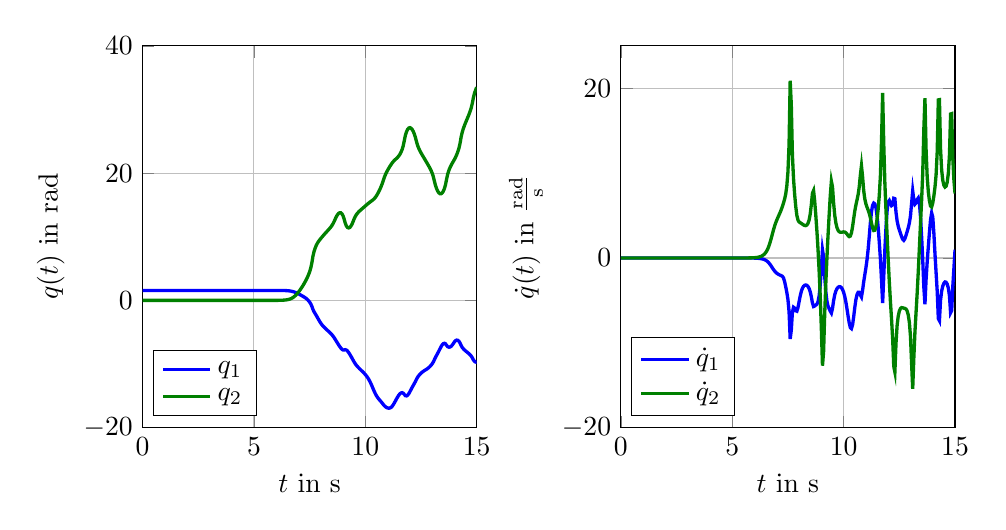
\begin{tikzpicture}

\begin{axis}[%
width=0.35\textwidth,
height=0.4\textwidth,
scale only axis,
xmin=0,
xmax=15,
xlabel={$t$ in $\mathrm{s}$},
xmajorgrids,
ymin=-20,
ymax=40,
ylabel={$q(t)$ in $\mathrm{rad}$},
ymajorgrids,
name=plot1,
legend style={at={(0.03,0.03)},anchor=south west,draw=black,fill=white,legend cell align=left}
]
\addplot [
color=blue,
solid,
line width=1.2pt
]
table[row sep=crcr]{
0 1.5707963267949\\
0.05 1.5707963267949\\
0.1 1.5707963267949\\
0.15 1.5707963267949\\
0.2 1.5707963267949\\
0.25 1.5707963267949\\
0.3 1.5707963267949\\
0.35 1.5707963267949\\
0.4 1.5707963267949\\
0.45 1.5707963267949\\
0.5 1.5707963267949\\
0.55 1.5707963267949\\
0.6 1.5707963267949\\
0.65 1.5707963267949\\
0.700000000000001 1.5707963267949\\
0.750000000000001 1.5707963267949\\
0.800000000000001 1.5707963267949\\
0.850000000000001 1.5707963267949\\
0.900000000000001 1.5707963267949\\
0.950000000000001 1.5707963267949\\
1 1.5707963267949\\
1.05 1.5707963267949\\
1.09999999999999 1.5707963267949\\
1.14999999999998 1.5707963267949\\
1.19999999999998 1.5707963267949\\
1.24999999999997 1.5707963267949\\
1.29999999999997 1.5707963267949\\
1.34999999999996 1.5707963267949\\
1.39999999999996 1.5707963267949\\
1.44999999999995 1.5707963267949\\
1.49999999999995 1.5707963267949\\
1.54999999999994 1.5707963267949\\
1.59999999999993 1.5707963267949\\
1.64999999999993 1.57079632679489\\
1.69999999999992 1.57079632679488\\
1.74999999999992 1.57079632679486\\
1.79999999999991 1.57079632679485\\
1.84999999999991 1.57079632679483\\
1.8999999999999 1.5707963267948\\
1.9499999999999 1.57079632679476\\
1.99999999999989 1.57079632679471\\
2.04999999999989 1.57079632679464\\
2.09999999999988 1.57079632679454\\
2.14999999999987 1.57079632679441\\
2.19999999999987 1.57079632679423\\
2.24999999999986 1.570796326794\\
2.29999999999986 1.57079632679369\\
2.34999999999985 1.57079632679326\\
2.39999999999985 1.5707963267927\\
2.44999999999984 1.57079632679195\\
2.49999999999984 1.57079632679093\\
2.54999999999983 1.57079632678958\\
2.59999999999982 1.57079632678777\\
2.64999999999982 1.57079632678535\\
2.69999999999981 1.57079632678211\\
2.74999999999981 1.57079632677778\\
2.7999999999998 1.570796326772\\
2.8499999999998 1.57079632676427\\
2.89999999999979 1.57079632675393\\
2.94999999999979 1.57079632674012\\
2.99999999999978 1.57079632672167\\
3.04999999999978 1.57079632669702\\
3.09999999999977 1.57079632666409\\
3.14999999999976 1.57079632662009\\
3.19999999999976 1.57079632656132\\
3.24999999999975 1.57079632648281\\
3.29999999999975 1.57079632637794\\
3.34999999999974 1.57079632623786\\
3.39999999999974 1.57079632605075\\
3.44999999999973 1.57079632580082\\
3.49999999999973 1.570796325467\\
3.54999999999972 1.57079632502113\\
3.59999999999971 1.57079632442559\\
3.64999999999971 1.57079632363017\\
3.6999999999997 1.57079632256778\\
3.7499999999997 1.57079632114882\\
3.79999999999969 1.57079631925363\\
3.84999999999969 1.57079631672238\\
3.89999999999968 1.57079631334163\\
3.94999999999968 1.57079630882627\\
3.99999999999967 1.57079630279557\\
4.04999999999969 1.57079629474096\\
4.0999999999997 1.57079628398326\\
4.14999999999972 1.57079626961534\\
4.19999999999974 1.57079625042566\\
4.24999999999975 1.5707962247961\\
4.29999999999977 1.57079619056553\\
4.34999999999979 1.57079614484759\\
4.3999999999998 1.57079608378727\\
4.44999999999982 1.57079600223594\\
4.49999999999984 1.57079589331712\\
4.54999999999985 1.57079574784672\\
4.59999999999987 1.57079555355863\\
4.64999999999989 1.57079529407045\\
4.6999999999999 1.5707949475021\\
4.74999999999992 1.57079448463096\\
4.79999999999994 1.57079386642775\\
4.84999999999995 1.57079304076568\\
4.89999999999997 1.57079193802508\\
4.94999999999999 1.57079046522315\\
5 1.57078849817366\\
5.05000000000002 1.57078587101562\\
5.10000000000004 1.570782362228\\
5.15000000000005 1.57077767595114\\
5.20000000000007 1.57077141704002\\
5.25000000000009 1.57076305774585\\
5.3000000000001 1.57075189321653\\
5.35000000000012 1.57073698206391\\
5.40000000000014 1.57071706698643\\
5.45000000000015 1.57069046875423\\
5.50000000000017 1.5706549446176\\
5.55000000000019 1.57060749920016\\
5.6000000000002 1.57054413193195\\
5.65000000000022 1.57045949972738\\
5.70000000000024 1.57034646646871\\
5.75000000000025 1.57019550131522\\
5.80000000000027 1.56999387512266\\
5.85000000000029 1.56972458725945\\
5.90000000000031 1.56936493243477\\
5.95000000000032 1.56888458694494\\
6.00000000000034 1.56824305356918\\
6.05000000000036 1.56738625109292\\
6.10000000000037 1.56624196427907\\
6.15000000000039 1.56471377870195\\
6.20000000000041 1.56267300823717\\
6.25000000000042 1.5599479801935\\
6.30000000000044 1.55630988297267\\
6.35000000000046 1.55145423934312\\
6.40000000000047 1.54497704666174\\
6.45000000000049 1.53634497917718\\
6.50000000000051 1.52486036452876\\
6.55000000000052 1.50962514803675\\
6.60000000000054 1.48951586850069\\
6.65000000000056 1.46319606157805\\
6.70000000000057 1.42921103122953\\
6.75000000000059 1.38621261970241\\
6.80000000000061 1.33330323918927\\
6.85000000000062 1.27035294651776\\
6.90000000000064 1.19806191977448\\
6.95000000000066 1.11769756413643\\
7.00000000000067 1.0307000227427\\
7.05000000000069 0.938394051292351\\
7.10000000000071 0.841878673048413\\
7.15000000000072 0.742019004557892\\
7.20000000000074 0.639369935584989\\
7.25000000000076 0.53362039299009\\
7.30000000000077 0.421624430140338\\
7.35000000000079 0.294399161753961\\
7.40000000000081 0.140472738021518\\
7.45000000000082 -0.0455812562394542\\
7.50000000000084 -0.268149726957854\\
7.55000000000086 -0.544592600930636\\
7.60000000000087 -0.932016264548337\\
7.65000000000089 -1.42072778604417\\
7.70000000000091 -1.78369587284048\\
7.75000000000092 -2.08465257456745\\
7.80000000000094 -2.37563586876921\\
7.85000000000096 -2.67902606722071\\
7.90000000000097 -2.99331796702977\\
7.95000000000099 -3.29803849024632\\
8.00000000000101 -3.5736095439324\\
8.05000000000098 -3.81384652512591\\
8.10000000000095 -4.02331829331435\\
8.15000000000092 -4.21027799978987\\
8.20000000000089 -4.38243576196293\\
8.25000000000087 -4.54589847164421\\
8.30000000000084 -4.70549137923492\\
8.35000000000081 -4.86538134050969\\
8.40000000000078 -5.02969990569745\\
8.45000000000076 -5.20320335435051\\
8.50000000000073 -5.39212310861744\\
8.5500000000007 -5.60516525351378\\
8.60000000000067 -5.85216756997586\\
8.65000000000065 -6.13033857121493\\
8.70000000000062 -6.41567985492126\\
8.75000000000059 -6.69575828190743\\
8.80000000000056 -6.97109041998317\\
8.85000000000053 -7.237689194783\\
8.90000000000051 -7.4804724678727\\
8.95000000000048 -7.67350973931384\\
9.00000000000045 -7.7848631878299\\
9.05000000000042 -7.7871456314419\\
9.1000000000004 -7.74298637274024\\
9.15000000000037 -7.7959565962644\\
9.20000000000034 -7.95349064356565\\
9.25000000000031 -8.18312952378009\\
9.30000000000028 -8.45432424928731\\
9.35000000000026 -8.74633045960232\\
9.40000000000023 -9.05228190815911\\
9.4500000000002 -9.3728392607445\\
9.50000000000017 -9.68754631327607\\
9.55000000000015 -9.96101595142577\\
9.60000000000012 -10.1937395493023\\
9.65000000000009 -10.3989248472928\\
9.70000000000006 -10.5863457854063\\
9.75000000000004 -10.7626898418914\\
9.80000000000001 -10.9330861792627\\
9.84999999999998 -11.1020343358109\\
9.89999999999995 -11.2739908134468\\
9.94999999999992 -11.4538348749514\\
9.9999999999999 -11.6472970164413\\
10.0499999999999 -11.8612781613053\\
10.0999999999998 -12.1037523113769\\
10.1499999999998 -12.3827022546398\\
10.1999999999998 -12.7037182600733\\
10.2499999999998 -13.0668810472135\\
10.2999999999997 -13.4643597459909\\
10.3499999999997 -13.8794178955955\\
10.3999999999997 -14.2871071035053\\
10.4499999999996 -14.6596027354059\\
10.4999999999996 -14.9789579045632\\
10.5499999999996 -15.2464097327286\\
10.5999999999996 -15.4759707952475\\
10.6499999999995 -15.6837840963943\\
10.6999999999995 -15.8847411847723\\
10.7499999999995 -16.0939534807076\\
10.7999999999995 -16.3209241819578\\
10.8499999999994 -16.5349445707446\\
10.8999999999994 -16.6999447260548\\
10.9499999999994 -16.8193209110082\\
10.9999999999993 -16.8979825287111\\
11.0499999999993 -16.9326793057314\\
11.0999999999993 -16.9131039774251\\
11.1499999999993 -16.824703666425\\
11.1999999999992 -16.6566718695072\\
11.2499999999992 -16.4141727059495\\
11.2999999999992 -16.1202252557286\\
11.3499999999991 -15.8016108941457\\
11.3999999999991 -15.4790261222317\\
11.4499999999991 -15.1702451097487\\
11.4999999999991 -14.8960892023531\\
11.549999999999 -14.6803700347525\\
11.599999999999 -14.5434450650222\\
11.649999999999 -14.4989179376322\\
11.699999999999 -14.563964531452\\
11.7499999999989 -14.7735715036445\\
11.7999999999989 -14.9738098681763\\
11.8499999999989 -15.0013968783495\\
11.8999999999988 -14.8870823075822\\
11.9499999999988 -14.6565986104239\\
11.9999999999988 -14.3484112847019\\
12.0499999999988 -14.0104779375126\\
12.0999999999987 -13.6784521181988\\
12.1499999999987 -13.3634406488408\\
12.1999999999987 -13.0546787709802\\
12.2499999999987 -12.724671441278\\
12.2999999999986 -12.3630458331155\\
12.3499999999986 -12.0543983125833\\
12.3999999999986 -11.812521673148\\
12.4499999999985 -11.6106016118044\\
12.4999999999985 -11.4350419742309\\
12.5499999999985 -11.2802186569835\\
12.5999999999985 -11.1443646756962\\
12.6499999999984 -11.0263656022107\\
12.6999999999984 -10.920447050577\\
12.7499999999984 -10.8127909204714\\
12.7999999999983 -10.6896921087925\\
12.8499999999983 -10.5456079649701\\
12.8999999999983 -10.3793150014366\\
12.9499999999983 -10.1879729162742\\
12.9999999999982 -9.96277971234112\\
13.0499999999982 -9.68173242124112\\
13.0999999999982 -9.3144816765918\\
13.1499999999982 -8.94215837627073\\
13.1999999999981 -8.61571409370913\\
13.2499999999981 -8.29703277298033\\
13.2999999999981 -7.9627442008694\\
13.349999999998 -7.61150398583219\\
13.399999999998 -7.26879658496705\\
13.449999999998 -6.98125369878372\\
13.499999999998 -6.79470549327005\\
13.5499999999979 -6.73569312085747\\
13.5999999999979 -6.82369707418454\\
13.6499999999979 -7.07362310112148\\
13.6999999999978 -7.27325957086048\\
13.7499999999978 -7.34578572747519\\
13.7999999999978 -7.32430475995193\\
13.8499999999978 -7.21682234997337\\
13.8999999999977 -7.02821967552024\\
13.9499999999977 -6.77910017453319\\
13.9999999999977 -6.5190177438956\\
14.0499999999977 -6.32057691817544\\
14.0999999999976 -6.23592038804891\\
14.1499999999976 -6.26895871757457\\
14.1999999999976 -6.40952349179554\\
14.2499999999975 -6.67938878463304\\
14.2999999999975 -7.08048575456699\\
14.3499999999975 -7.3813354884823\\
14.3999999999975 -7.59884983323119\\
14.4499999999974 -7.77722852989872\\
14.4999999999974 -7.93391770231877\\
14.5499999999974 -8.07831583872546\\
14.5999999999973 -8.21962526785283\\
14.6499999999973 -8.36758969745526\\
14.6999999999973 -8.53232735693036\\
14.7499999999973 -8.73033161923047\\
14.7999999999972 -8.99850715415883\\
14.8499999999972 -9.34334375443183\\
14.8999999999972 -9.57750397023928\\
14.9499999999972 -9.68976112859502\\
14.9999999999971 -9.69665386240826\\
};
\addlegendentry{$q_1$};

\addplot [
color=green!50!black,
solid,
line width=1.2pt
]
table[row sep=crcr]{
0 0\\
0.05 7.55476594189969e-19\\
0.1 3.0778322046573e-18\\
0.15 7.13898434835287e-18\\
0.2 1.32395688061868e-17\\
0.25 2.18311948524722e-17\\
0.3 3.35498766315504e-17\\
0.35 4.92631155132876e-17\\
0.4 7.01341188030717e-17\\
0.45 9.77079087385312e-17\\
0.5 1.34025696182147e-16\\
0.55 1.81775985775635e-16\\
0.6 2.44493598449777e-16\\
0.65 3.26821344371727e-16\\
0.700000000000001 4.34853717249198e-16\\
0.750000000000001 5.76588052723508e-16\\
0.800000000000001 7.62516548850633e-16\\
0.850000000000001 1.0064029742974e-15\\
0.900000000000001 1.3263015617971e-15\\
0.950000000000001 1.74589351270889e-15\\
1 2.29624005039072e-15\\
1.05 3.0180817960439e-15\\
1.09999999999999 3.96485468341814e-15\\
1.14999999999998 5.20664567214191e-15\\
1.19999999999998 6.83538109011742e-15\\
1.24999999999997 8.97163168351562e-15\\
1.29999999999997 1.17735381332669e-14\\
1.34999999999996 1.54485177691716e-14\\
1.39999999999996 2.02686190970667e-14\\
1.44999999999995 2.65906607919253e-14\\
1.49999999999995 3.48826459904511e-14\\
1.54999999999994 4.57584072596716e-14\\
1.59999999999993 6.00230469120526e-14\\
1.64999999999993 7.87692719078785e-14\\
1.69999999999992 1.03604323164006e-13\\
1.74999999999992 1.3664167768029e-13\\
1.79999999999991 1.80602090286411e-13\\
1.84999999999991 2.39109895497064e-13\\
1.8999999999999 3.17042492434978e-13\\
1.9499999999999 4.20887623269642e-13\\
1.99999999999989 5.59307327975818e-13\\
2.04999999999989 7.43866191106113e-13\\
2.09999999999988 9.90005436115027e-13\\
2.14999999999987 1.31834071742812e-12\\
2.19999999999987 1.75639998699398e-12\\
2.24999999999986 2.34094750979144e-12\\
2.29999999999986 3.12107438257363e-12\\
2.34999999999985 4.16233932497804e-12\\
2.39999999999985 5.55228977054502e-12\\
2.44999999999984 7.40783416188817e-12\\
2.49999999999984 9.8851049281432e-12\\
2.54999999999983 1.31926161447885e-11\\
2.59999999999982 1.76088418456711e-11\\
2.64999999999982 2.35056936262048e-11\\
2.69999999999981 3.13798641044277e-11\\
2.74999999999981 4.18947038746139e-11\\
2.7999999999998 5.59361481885684e-11\\
2.8499999999998 7.46874119969691e-11\\
2.89999999999979 9.97287434028141e-11\\
2.94999999999979 1.33170671727761e-10\\
2.99999999999978 1.77831947206996e-10\\
3.04999999999978 2.37477181303123e-10\\
3.09999999999977 3.17134263757445e-10\\
3.14999999999976 4.23518291866223e-10\\
3.19999999999976 5.65597768185967e-10\\
3.24999999999975 7.55350801326742e-10\\
3.29999999999975 1.00877505790393e-09\\
3.34999999999974 1.34723664799159e-09\\
3.39999999999974 1.79927166931002e-09\\
3.44999999999973 2.40299230646389e-09\\
3.49999999999973 3.20930040943542e-09\\
3.54999999999972 4.28617945502795e-09\\
3.59999999999971 5.72442680368359e-09\\
3.64999999999971 7.64530961462732e-09\\
3.6999999999997 1.02107899941033e-08\\
3.7499999999997 1.3637181448502e-08\\
3.79999999999969 1.8213388238566e-08\\
3.84999999999969 2.43252655365004e-08\\
3.89999999999968 3.24881544258045e-08\\
3.94999999999968 4.33903350803729e-08\\
3.99999999999967 5.79510620367902e-08\\
4.04999999999969 7.73980750880038e-08\\
4.0999999999997 1.03371121515075e-07\\
4.14999999999972 1.38060218555046e-07\\
4.19999999999974 1.84390314283908e-07\\
4.24999999999975 2.46267917492351e-07\\
4.29999999999977 3.28910492243669e-07\\
4.34999999999979 4.39286391446737e-07\\
4.3999999999998 5.86702424492187e-07\\
4.44999999999982 7.83588602289391e-07\\
4.49999999999984 1.04654622901498e-06\\
4.54999999999985 1.39774771518111e-06\\
4.59999999999987 1.86680614350545e-06\\
4.64999999999989 2.49327222841379e-06\\
4.6999999999999 3.32996921159592e-06\\
4.74999999999992 4.44744689024101e-06\\
4.79999999999994 5.93993033943348e-06\\
4.84999999999995 7.93326492191069e-06\\
4.89999999999997 1.05955275044073e-05\\
4.94999999999999 1.41511986130023e-05\\
5 1.89000905163765e-05\\
5.05000000000002 2.52426272433312e-05\\
5.10000000000004 3.37136081326666e-05\\
5.15000000000005 4.50273018403966e-05\\
5.20000000000007 6.01376731069198e-05\\
5.25000000000009 8.03188205716982e-05\\
5.3000000000001 0.000107272408103947\\
5.35000000000012 0.000143271148187231\\
5.40000000000014 0.000191350435762133\\
5.45000000000015 0.000255564290894745\\
5.50000000000017 0.000341327190986452\\
5.55000000000019 0.000455870615069409\\
5.6000000000002 0.000608852794401959\\
5.65000000000022 0.000813173079961007\\
5.70000000000024 0.00108605958610704\\
5.75000000000025 0.0014505218014498\\
5.80000000000027 0.00193729060616628\\
5.85000000000029 0.00258740917183794\\
5.90000000000031 0.0034556929565189\\
5.95000000000032 0.00461534994295114\\
6.00000000000034 0.00616414927366946\\
6.05000000000036 0.00823265503116695\\
6.10000000000037 0.0109952113627471\\
6.15000000000039 0.0146845860007079\\
6.20000000000041 0.0196114612023439\\
6.25000000000042 0.0261903069102811\\
6.30000000000044 0.0349735598469859\\
6.35000000000046 0.0466963802637424\\
6.40000000000047 0.0623343239391033\\
6.45000000000049 0.0831754440562133\\
6.50000000000051 0.110905229729418\\
6.55000000000052 0.147694494366957\\
6.60000000000054 0.196261809685611\\
6.65000000000056 0.259847982666607\\
6.70000000000057 0.34199637137267\\
6.75000000000059 0.446027329264933\\
6.80000000000061 0.574235477386351\\
6.85000000000062 0.727161862268716\\
6.90000000000064 0.903484719397437\\
6.95000000000066 1.10069521712685\\
7.00000000000067 1.31609608981624\\
7.05000000000069 1.5475628765239\\
7.10000000000071 1.79390160833791\\
7.15000000000072 2.05494077238764\\
7.20000000000074 2.33151806845502\\
7.25000000000076 2.6253718325798\\
7.30000000000077 2.93870121022263\\
7.35000000000079 3.27359703907235\\
7.40000000000081 3.63434303040433\\
7.45000000000082 4.03329011176986\\
7.50000000000084 4.49563980257691\\
7.55000000000086 5.07400976358981\\
7.60000000000087 5.90846277060787\\
7.65000000000089 6.97209737701569\\
7.70000000000091 7.70665955284345\\
7.75000000000092 8.23821292536621\\
7.80000000000094 8.65804400458076\\
7.85000000000096 8.99620665238404\\
7.90000000000097 9.27144570246499\\
7.95000000000099 9.50686365998907\\
8.00000000000101 9.72376477140898\\
8.05000000000098 9.93359342161246\\
8.10000000000095 10.1394018032587\\
8.15000000000092 10.3409384551705\\
8.20000000000089 10.5378406413568\\
8.25000000000087 10.7307240634117\\
8.30000000000084 10.9214595561208\\
8.35000000000081 11.1133937339958\\
8.40000000000078 11.3118024218299\\
8.45000000000076 11.5247513417321\\
8.50000000000073 11.764555887196\\
8.5500000000007 12.0494122760389\\
8.60000000000067 12.3985268106716\\
8.65000000000065 12.7956479380481\\
8.70000000000062 13.1662580085325\\
8.75000000000059 13.4611870343424\\
8.80000000000056 13.6671607993605\\
8.85000000000053 13.7727117798325\\
8.90000000000051 13.7609231660543\\
8.95000000000048 13.6104291413012\\
9.00000000000045 13.2906526099959\\
9.05000000000042 12.7584435514794\\
9.1000000000004 12.1314552902071\\
9.15000000000037 11.6942731450998\\
9.20000000000034 11.4590222567663\\
9.25000000000031 11.3875575733556\\
9.30000000000028 11.4572868516222\\
9.35000000000026 11.6523352267522\\
9.40000000000023 11.9634927172961\\
9.4500000000002 12.3789998564838\\
9.50000000000017 12.8256640997308\\
9.55000000000015 13.196494645122\\
9.60000000000012 13.4818232497817\\
9.65000000000009 13.7095856443601\\
9.70000000000006 13.9015264779407\\
9.75000000000004 14.0718965967847\\
9.80000000000001 14.2301903354382\\
9.84999999999998 14.3828004399505\\
9.89999999999995 14.5338674530862\\
9.94999999999992 14.6856883052697\\
9.9999999999999 14.8388668317385\\
10.0499999999999 14.9923340937795\\
10.0999999999998 15.1434614537675\\
10.1499999999998 15.2887037175867\\
10.1999999999998 15.4252622093405\\
10.2499999999998 15.5536443304763\\
10.2999999999997 15.6799828541853\\
10.3499999999997 15.8167943296553\\
10.3999999999997 15.9810641925917\\
10.4499999999996 16.1879945244711\\
10.4999999999996 16.442277772373\\
10.5499999999996 16.7371797772707\\
10.5999999999996 17.0640912289906\\
10.6499999999995 17.4208865272953\\
10.6999999999995 17.8152718716251\\
10.7499999999995 18.2666636075234\\
10.7999999999995 18.7892217806696\\
10.8499999999994 19.3084659024671\\
10.8999999999994 19.7440126055076\\
10.9499999999994 20.1143571471127\\
10.9999999999993 20.4464513943849\\
11.0499999999993 20.7548127074415\\
11.0999999999993 21.0454733522096\\
11.1499999999993 21.318359798593\\
11.1999999999992 21.5686245183049\\
11.2499999999992 21.790036408064\\
11.2999999999992 21.9812401914774\\
11.3499999999991 22.1497566826231\\
11.3999999999991 22.3106454898398\\
11.4499999999991 22.4833159853886\\
11.4999999999991 22.6884933144382\\
11.549999999999 22.9454712931125\\
11.599999999999 23.2724089177072\\
11.649999999999 23.6945877539317\\
11.699999999999 24.2692730158376\\
11.7499999999989 25.1182513184974\\
11.7999999999989 25.9641626369566\\
11.8499999999989 26.5128829344001\\
11.8999999999988 26.8721392047548\\
11.9499999999988 27.0797834705089\\
11.9999999999988 27.1421784815948\\
12.0499999999988 27.066063915399\\
12.0999999999987 26.8662425916119\\
12.1499999999987 26.5579063730503\\
12.1999999999987 26.1415166145459\\
12.2499999999987 25.5870148541144\\
12.2999999999986 24.9026702366127\\
12.3499999999986 24.316678490642\\
12.3999999999986 23.8719738868163\\
12.4499999999985 23.5046529335535\\
12.4999999999985 23.1786990935145\\
12.5499999999985 22.8745611153864\\
12.5999999999985 22.580125199835\\
12.6499999999984 22.2875402599986\\
12.6999999999984 21.9930211970764\\
12.7499999999984 21.6966108220147\\
12.7999999999983 21.3980277309053\\
12.8499999999983 21.0924155219406\\
12.8999999999983 20.7698706407279\\
12.9499999999983 20.4144680425933\\
12.9999999999982 19.9985017715525\\
13.0499999999982 19.4661779922492\\
13.0999999999982 18.7479676426809\\
13.1499999999982 18.0570500081876\\
13.1999999999981 17.5489530763552\\
13.2499999999981 17.1713245638913\\
13.2999999999981 16.9058080500332\\
13.349999999998 16.7607822605563\\
13.399999999998 16.7504631210926\\
13.449999999998 16.8816557374425\\
13.499999999998 17.1528294842085\\
13.5499999999979 17.5700797692073\\
13.5999999999979 18.1870265107798\\
13.6499999999979 19.092429058549\\
13.6999999999978 19.8768329261126\\
13.7499999999978 20.4265208733901\\
13.7999999999978 20.8576073016464\\
13.8499999999978 21.2198532755822\\
13.8999999999977 21.5397411051372\\
13.9499999999977 21.8408190254576\\
13.9999999999977 22.1505905500672\\
14.0499999999977 22.4936283553254\\
14.0999999999976 22.8835132837934\\
14.1499999999976 23.3343582051305\\
14.1999999999976 23.8840865645666\\
14.2499999999975 24.6418685144855\\
14.2999999999975 25.6596194982663\\
14.3499999999975 26.4272183579613\\
14.3999999999975 26.9989053246086\\
14.4499999999974 27.4829412171378\\
14.4999999999974 27.92370110971\\
14.5499999999974 28.3452635589054\\
14.5999999999973 28.7644444606276\\
14.6499999999973 29.1975845621712\\
14.6999999999973 29.6672570171098\\
14.7499999999973 30.2138957062124\\
14.7999999999972 30.9285104305621\\
14.8499999999972 31.8412909297093\\
14.8999999999972 32.5463182766545\\
14.9499999999972 33.0624672556325\\
14.9999999999971 33.4796516310256\\
};
\addlegendentry{$q_2$};

\end{axis}

\begin{axis}[%
width=0.35\textwidth,
height=0.4\textwidth,
scale only axis,
xmin=0,
xmax=15,
xlabel={$t$ in $\mathrm{s}$},
xmajorgrids,
ymin=-20,
ymax=25,
ylabel={$\dot{q}(t)$ in $\mathrm{\frac{rad}{s}}$},
ymajorgrids,
at=(plot1.right of south east),
anchor=left of south west,
legend style={at={(0.03,0.03)},anchor=south west,draw=black,fill=white,legend cell align=left}
]
\addplot [
color=blue,
solid,
line width=1.2pt
]
table[row sep=crcr]{
0 0\\
0.05 -3.00344627490888e-17\\
0.1 -6.00689254981777e-17\\
0.15 -9.01033882472665e-17\\
0.2 -1.20137850996355e-16\\
0.25 -1.50172313745445e-16\\
0.3 -1.80206776494534e-16\\
0.35 -2.10241239243624e-16\\
0.4 -2.76717535020441e-16\\
0.45 -3.61208437127393e-16\\
0.5 -4.45699339234346e-16\\
0.55 -5.45938627413041e-16\\
0.6 -6.84885968877859e-16\\
0.65 -8.54829499434618e-16\\
0.700000000000001 -1.06991658644953e-15\\
0.750000000000001 -1.34550560936054e-15\\
0.800000000000001 -1.70208016915499e-15\\
0.850000000000001 -2.16261260071348e-15\\
0.900000000000001 -2.76098505812367e-15\\
0.950000000000001 -3.53945377204861e-15\\
1 -4.55487459225596e-15\\
1.05 -5.88023988820852e-15\\
1.09999999999999 -7.61312532902268e-15\\
1.14999999999998 -9.87886474311637e-15\\
1.19999999999998 -1.28452273181687e-14\\
1.24999999999997 -1.67293228935238e-14\\
1.29999999999997 -2.18157488316344e-14\\
1.34999999999996 -2.84809353842357e-14\\
1.39999999999996 -3.72169302180482e-14\\
1.44999999999995 -4.86701651582702e-14\\
1.49999999999995 -6.36854080899543e-14\\
1.54999999999994 -8.33686391983283e-14\\
1.59999999999993 -1.09182548062715e-13\\
1.64999999999993 -1.4540171093257e-13\\
1.69999999999992 -1.97705087855155e-13\\
1.74999999999992 -2.69550303287532e-13\\
1.79999999999991 -3.65833253746964e-13\\
1.84999999999991 -4.96657212994497e-13\\
1.8999999999999 -6.72718236106629e-13\\
1.9499999999999 -9.09772922160428e-13\\
1.99999999999989 -1.22824127853992e-12\\
2.04999999999989 -1.65575114660701e-12\\
2.09999999999988 -2.22902962773299e-12\\
2.14999999999987 -2.99723449662446e-12\\
2.19999999999987 -4.02615793843131e-12\\
2.24999999999986 -5.40367400227815e-12\\
2.29999999999986 -7.24705181839076e-12\\
2.34999999999985 -9.7131816877556e-12\\
2.39999999999985 -1.301131630817e-11\\
2.44999999999984 -1.74211947017823e-11\\
2.49999999999984 -2.33165766366848e-11\\
2.54999999999983 -3.11967743994738e-11\\
2.59999999999982 -4.17286002761207e-11\\
2.64999999999982 -5.5802868461059e-11\\
2.69999999999981 -7.46093054676982e-11\\
2.74999999999981 -9.97370275534662e-11\\
2.7999999999998 -1.33308756168549e-10\\
2.8499999999998 -1.78159659926547e-10\\
2.89999999999979 -2.38076534578443e-10\\
2.94999999999979 -3.1811746414736e-10\\
2.99999999999978 -4.25037615943333e-10\\
3.04999999999978 -5.67859226664397e-10\\
3.09999999999977 -7.5863285835962e-10\\
3.14999999999976 -1.01345300221917e-09\\
3.19999999999976 -1.35381639738813e-09\\
3.24999999999975 -1.8084334998558e-09\\
3.29999999999975 -2.41565020121571e-09\\
3.34999999999974 -3.22668118173315e-09\\
3.39999999999974 -4.3099282799877e-09\\
3.44999999999973 -5.75674870881227e-09\\
3.49999999999973 -7.68915860917253e-09\\
3.54999999999972 -1.02701211706486e-08\\
3.59999999999971 -1.37172877382124e-08\\
3.64999999999971 -1.83213513594545e-08\\
3.6999999999997 -2.44705579806039e-08\\
3.7499999999997 -3.26834430375861e-08\\
3.79999999999969 -4.36525551938561e-08\\
3.84999999999969 -5.83028523178369e-08\\
3.89999999999968 -7.78696941567504e-08\\
3.94999999999968 -1.04003007966838e-07\\
3.99999999999967 -1.38906410070547e-07\\
4.04999999999969 -1.85523014660682e-07\\
4.0999999999997 -2.47783598122538e-07\\
4.14999999999972 -3.30938040049033e-07\\
4.19999999999974 -4.4199799182343e-07\\
4.24999999999975 -5.90328097788713e-07\\
4.29999999999977 -7.88435618592683e-07\\
4.34999999999979 -1.05302503948429e-06\\
4.3999999999998 -1.40640658627544e-06\\
4.44999999999982 -1.87837741501045e-06\\
4.49999999999984 -2.50873409543656e-06\\
4.54999999999985 -3.35062824257635e-06\\
4.59999999999987 -4.47504823613571e-06\\
4.64999999999989 -5.97680493029228e-06\\
4.6999999999999 -7.98252606123431e-06\\
4.74999999999992 -1.0661333440047e-05\\
4.79999999999994 -1.42391032240297e-05\\
4.84999999999995 -1.90175116878498e-05\\
4.89999999999997 -2.53994724221451e-05\\
4.94999999999999 -3.39231098137269e-05\\
5 -4.53071334313623e-05\\
5.05000000000002 -6.05114392637954e-05\\
5.10000000000004 -8.08180476740318e-05\\
5.15000000000005 -0.000107939202713292\\
5.20000000000007 -0.00014416174766487\\
5.25000000000009 -0.000192539950468741\\
5.3000000000001 -0.000257153037915235\\
5.35000000000012 -0.000343449153631663\\
5.40000000000014 -0.000458704741915309\\
5.45000000000015 -0.000612638091687523\\
5.50000000000017 -0.000818228772526152\\
5.55000000000019 -0.00109281205301115\\
5.6000000000002 -0.00145954057218788\\
5.65000000000022 -0.0019493364877241\\
5.70000000000024 -0.00260349864815165\\
5.75000000000025 -0.00347718448941084\\
5.80000000000027 -0.00464405992530136\\
5.85000000000029 -0.00620250854076877\\
5.90000000000031 -0.00828392181572463\\
5.95000000000032 -0.0110637650515328\\
6.00000000000034 -0.0147763416993775\\
6.05000000000036 -0.0197344763047151\\
6.10000000000037 -0.0263557169000806\\
6.15000000000039 -0.0351971262344168\\
6.20000000000041 -0.0470012625846914\\
6.25000000000042 -0.0627564371062961\\
6.30000000000044 -0.0837744581317361\\
6.35000000000046 -0.111788011921425\\
6.40000000000047 -0.149065605717747\\
6.45000000000049 -0.198530140114754\\
6.50000000000051 -0.263838418269758\\
6.55000000000052 -0.34931703274626\\
6.60000000000054 -0.459537866364337\\
6.65000000000056 -0.598177957774585\\
6.70000000000057 -0.765838929028524\\
6.75000000000059 -0.957208562695357\\
6.80000000000061 -1.15962540235197\\
6.85000000000062 -1.35595290527282\\
6.90000000000064 -1.53131858356586\\
6.95000000000066 -1.67835637206392\\
7.00000000000067 -1.79709698934657\\
7.05000000000069 -1.8914828659146\\
7.10000000000071 -1.96623899650713\\
7.15000000000072 -2.02615954005351\\
7.20000000000074 -2.08024198817428\\
7.25000000000076 -2.15883115980064\\
7.30000000000077 -2.35162938073588\\
7.35000000000079 -2.7804029435518\\
7.40000000000081 -3.39204016115503\\
7.45000000000082 -4.06018050519924\\
7.50000000000084 -4.89341885973917\\
7.55000000000086 -6.33362876473385\\
7.60000000000087 -9.54353873383308\\
7.65000000000089 -8.52190186478511\\
7.70000000000091 -6.38793190088129\\
7.75000000000092 -5.80805042030209\\
7.80000000000094 -5.90643258454013\\
7.85000000000096 -6.22361761030134\\
7.90000000000097 -6.2712519663092\\
7.95000000000099 -5.84795601783538\\
8.00000000000101 -5.15586924098735\\
8.05000000000098 -4.47154333066737\\
8.10000000000095 -3.93620687805846\\
8.15000000000092 -3.56813047056544\\
8.20000000000089 -3.33838126351498\\
8.25000000000087 -3.21599318083226\\
8.30000000000084 -3.18140807808404\\
8.35000000000081 -3.22775043235139\\
8.40000000000078 -3.36057024842652\\
8.45000000000076 -3.59995329739515\\
8.50000000000073 -3.98578427152707\\
8.5500000000007 -4.57276619451588\\
8.60000000000067 -5.30737685808943\\
8.65000000000065 -5.71802023503138\\
8.70000000000062 -5.65872125289582\\
8.75000000000059 -5.55249633448968\\
8.80000000000056 -5.44933396193144\\
8.85000000000053 -5.16427422682067\\
8.90000000000051 -4.45870070676456\\
8.95000000000048 -3.15455144934249\\
9.00000000000045 -1.19122561997038\\
9.05000000000042 0.968325443793873\\
9.1000000000004 0.13898960294892\\
9.15000000000037 -2.20638316966192\\
9.20000000000034 -3.9824277365818\\
9.25000000000031 -5.09858433859944\\
9.30000000000028 -5.67845882250702\\
9.35000000000026 -5.98023022665143\\
9.40000000000023 -6.2702495018007\\
9.4500000000002 -6.4916006949613\\
9.50000000000017 -5.94307497569884\\
9.55000000000015 -5.01671871433417\\
9.60000000000012 -4.33950425146737\\
9.65000000000009 -3.8998604519022\\
9.70000000000006 -3.61874858602266\\
9.75000000000004 -3.45181900997937\\
9.80000000000001 -3.37884773075679\\
9.84999999999998 -3.39378231304855\\
9.89999999999995 -3.50059552435737\\
9.94999999999992 -3.71214824955907\\
9.9999999999999 -4.0493438866939\\
10.0499999999999 -4.5368100617586\\
10.0999999999998 -5.18959414390712\\
10.1499999999998 -5.9881646546379\\
10.1999999999998 -6.8535792819927\\
10.2499999999998 -7.6471372959832\\
10.2999999999997 -8.19612510210469\\
10.3499999999997 -8.3215730062389\\
10.3999999999997 -7.88843091628083\\
10.4499999999996 -6.9474122616917\\
10.4999999999996 -5.83405600258184\\
10.5499999999996 -4.91488427790422\\
10.5999999999996 -4.3222429939542\\
10.6499999999995 -4.03911219415278\\
10.6999999999995 -4.0495216936445\\
10.7499999999995 -4.36587399479405\\
10.7999999999995 -4.6019648911468\\
10.8499999999994 -3.8168251864433\\
10.8999999999994 -2.81419940983322\\
10.9499999999994 -1.97796336235776\\
10.9999999999993 -1.1571952662139\\
11.0499999999993 -0.195619695066572\\
11.0999999999993 1.02969775360217\\
11.1499999999993 2.54730983126224\\
11.1999999999992 4.15801668364623\\
11.2499999999992 5.45892688137311\\
11.2999999999992 6.20604881120808\\
11.3499999999991 6.4713104368079\\
11.3999999999991 6.37524693525656\\
11.4499999999991 5.9066387480601\\
11.4999999999991 4.97751829228721\\
11.549999999999 3.58171442142228\\
11.599999999999 1.85320451921476\\
11.649999999999 -0.119687972038304\\
11.699999999999 -2.63115392599248\\
11.7499999999989 -5.32058140245558\\
11.7999999999989 -2.19193760146333\\
11.8499999999989 0.953985103768974\\
11.8999999999988 3.54506168656643\\
11.9499999999988 5.54385956259186\\
11.9999999999988 6.61481179661631\\
12.0499999999988 6.77941954469346\\
12.0999999999987 6.46637825402676\\
12.1499999999987 6.17181984563407\\
12.1999999999987 6.27213945555956\\
12.2499999999987 7.03288003864926\\
12.2999999999986 6.98595222792141\\
12.3499999999986 5.39691629365264\\
12.3999999999986 4.37276382710322\\
12.4499999999985 3.74656243598359\\
12.4999999999985 3.2933914228168\\
12.5499999999985 2.90454589036463\\
12.5999999999985 2.53147575502581\\
12.6499999999984 2.20569091200853\\
12.6999999999984 2.08068366560218\\
12.7499999999984 2.27481937203104\\
12.7999999999983 2.66537818270754\\
12.8499999999983 3.10002275371221\\
12.8999999999983 3.55997287758128\\
12.9499999999983 4.12091637178179\\
12.9999999999982 4.95538971039926\\
13.0499999999982 6.43489505831656\\
13.0999999999982 7.91064765715895\\
13.1499999999982 6.867061701898\\
13.1999999999981 6.33940752515238\\
13.2499999999981 6.4854040989597\\
13.2999999999981 6.89330861473058\\
13.349999999998 7.06985212591516\\
13.399999999998 6.47464272846655\\
13.449999999998 4.86638518661993\\
13.499999999998 2.51121453084492\\
13.5499999999979 -0.199601439344769\\
13.5999999999979 -3.47881068521304\\
13.6499999999979 -5.45011350324791\\
13.6999999999978 -2.5547474149675\\
13.7499999999978 -0.456802638685699\\
13.7999999999978 1.29738854343592\\
13.8499999999978 2.99188609760151\\
13.8999999999977 4.48842056956779\\
13.9499999999977 5.31113795690442\\
13.9999999999977 4.83264594657875\\
14.0499999999977 2.91763766774701\\
14.0999999999976 0.472257522008314\\
14.1499999999976 -1.74557897023951\\
14.1999999999976 -3.93282790331049\\
14.2499999999975 -7.14251550964645\\
14.2999999999975 -7.39312809462906\\
14.3499999999975 -4.95769389688384\\
14.3999999999975 -3.87525285616772\\
14.4499999999974 -3.31302110776148\\
14.4999999999974 -2.98312893784\\
14.5499999999974 -2.82360909435852\\
14.5999999999973 -2.86169379396119\\
14.6499999999973 -3.08853142568736\\
14.6999999999973 -3.5517367710865\\
14.7499999999973 -4.48306425233801\\
14.7999999999972 -6.45809760530652\\
14.8499999999972 -6.20423397313466\\
14.8999999999972 -3.33493648151687\\
14.9499999999972 -1.20078767140397\\
14.9999999999971 0.968413087722353\\
};
\addlegendentry{$\dot{q}_1$};

\addplot [
color=green!50!black,
solid,
line width=1.2pt
]
table[row sep=crcr]{
0 0\\
0.05 3.04041175992209e-17\\
0.1 6.30589673340292e-17\\
0.15 1.00381896770624e-16\\
0.2 1.45135818412652e-16\\
0.25 2.00633740417792e-16\\
0.3 2.70984019363329e-16\\
0.35 3.61394490439794e-16\\
0.4 4.7855798898376e-16\\
0.45 6.31147802435003e-16\\
0.5 8.30459729646332e-16\\
0.55 1.09124827740837e-15\\
0.6 1.43281889548874e-15\\
0.65 1.88045710530334e-15\\
0.700000000000001 2.4673003166342e-15\\
0.750000000000001 3.23679089777183e-15\\
0.800000000000001 4.24589209303163e-15\\
0.850000000000001 5.56930485306015e-15\\
0.900000000000001 7.30499773813287e-15\\
0.950000000000001 9.58145925778129e-15\\
1 1.25672095172504e-14\\
1.05 1.64832752914792e-14\\
1.09999999999999 2.16195520215826e-14\\
1.14999999999998 2.83562639668565e-14\\
1.19999999999998 3.71921111475842e-14\\
1.24999999999997 4.8781186718415e-14\\
1.29999999999997 6.39813976626349e-14\\
1.34999999999996 8.39179732564502e-14\\
1.39999999999996 1.10066762657993e-13\\
1.44999999999995 1.4436348790954e-13\\
1.49999999999995 1.89347040048371e-13\\
1.54999999999994 2.48347426138211e-13\\
1.59999999999993 3.25732280416466e-13\\
1.64999999999993 4.29603976798914e-13\\
1.69999999999992 5.70788137219742e-13\\
1.74999999999992 7.5970525965023e-13\\
1.79999999999991 1.01057347028411e-12\\
1.84999999999991 1.34589951226551e-12\\
1.8999999999999 1.79292975552616e-12\\
1.9499999999999 2.38950445325749e-12\\
1.99999999999989 3.18551025384153e-12\\
2.04999999999989 4.24788801484394e-12\\
2.09999999999988 5.66584507342771e-12\\
2.14999999999987 7.55856599918244e-12\\
2.19999999999987 1.00853346107095e-11\\
2.24999999999986 1.34588309098794e-11\\
2.29999999999986 1.79629468939589e-11\\
2.34999999999985 2.39770411151044e-11\\
2.39999999999985 3.20074232327335e-11\\
2.44999999999984 4.27304770050747e-11\\
2.49999999999984 5.7049599426764e-11\\
2.54999999999983 7.61713666827655e-11\\
2.59999999999982 1.01707073491503e-10\\
2.64999999999982 1.35808827066738e-10\\
2.69999999999981 1.81350737273448e-10\\
2.74999999999981 2.42171374041966e-10\\
2.7999999999998 3.23397587407671e-10\\
2.8499999999998 4.3187655462086e-10\\
2.89999999999979 5.76753195843752e-10\\
2.94999999999979 7.70241507059799e-10\\
2.99999999999978 1.02865365202525e-09\\
3.04999999999978 1.37377567144742e-09\\
3.09999999999977 1.83470479242986e-09\\
3.14999999999976 2.45030226573485e-09\\
3.19999999999976 3.27247115450061e-09\\
3.24999999999975 4.3705314633076e-09\\
3.29999999999975 5.8370657881195e-09\\
3.34999999999974 7.79572563688235e-09\\
3.39999999999974 1.04116573356224e-08\\
3.44999999999973 1.39054273464483e-08\\
3.49999999999973 1.85716203248276e-08\\
3.54999999999972 2.48036777045289e-08\\
3.59999999999971 3.31270721528141e-08\\
3.64999999999971 4.42436159000156e-08\\
3.6999999999997 5.90906367043196e-08\\
3.7499999999997 7.89200120705331e-08\\
3.79999999999969 1.05403727243614e-07\\
3.84999999999969 1.40774855917829e-07\\
3.89999999999968 1.88015851620418e-07\\
3.94999999999968 2.51110026286957e-07\\
3.99999999999967 3.35377420435604e-07\\
4.04999999999969 4.47923385875781e-07\\
4.0999999999997 5.98237706225664e-07\\
4.14999999999972 7.98994768870202e-07\\
4.19999999999974 1.06712226231794e-06\\
4.24999999999975 1.42522851037731e-06\\
4.29999999999977 1.90350879334994e-06\\
4.34999999999979 2.54229139838026e-06\\
4.3999999999998 3.39543807928851e-06\\
4.44999999999982 4.53488565157691e-06\\
4.49999999999984 6.05671166667203e-06\\
4.54999999999985 8.08923562291865e-06\\
4.59999999999987 1.08038387979068e-05\\
4.64999999999989 1.44294150310146e-05\\
4.6999999999999 1.92716709341797e-05\\
4.74999999999992 2.57389029180207e-05\\
4.79999999999994 3.43764245366212e-05\\
4.84999999999995 4.59125470497175e-05\\
4.89999999999997 6.13199902577007e-05\\
4.94999999999999 8.18979017422419e-05\\
5 0.000109381400330214\\
5.05000000000002 0.000146087880430835\\
5.10000000000004 0.000195112413549694\\
5.15000000000005 0.00026058872312695\\
5.20000000000007 0.00034803773794377\\
5.25000000000009 0.000464833113890427\\
5.3000000000001 0.000620822976527084\\
5.35000000000012 0.000829160309147189\\
5.40000000000014 0.0011074120035074\\
5.45000000000015 0.00147904008606342\\
5.50000000000017 0.00197538001177005\\
5.55000000000019 0.0026382828241901\\
5.6000000000002 0.00352364394372007\\
5.65000000000022 0.00470611607287018\\
5.70000000000024 0.00628540347330041\\
5.75000000000025 0.00839466802301652\\
5.80000000000027 0.0112117550814506\\
5.85000000000029 0.0149741838949902\\
5.90000000000031 0.0199991621746963\\
5.95000000000032 0.0267103020990252\\
6.00000000000034 0.035673265729772\\
6.05000000000036 0.0476432866403292\\
6.10000000000037 0.0636284347490494\\
6.15000000000039 0.0849736256392709\\
6.20000000000041 0.113471665817317\\
6.25000000000042 0.15150881664944\\
6.30000000000044 0.202252699138821\\
6.35000000000046 0.269887897975851\\
6.40000000000047 0.359894654409301\\
6.45000000000049 0.4793379322502\\
6.50000000000051 0.637065883786065\\
6.55000000000052 0.843569878205367\\
6.60000000000054 1.10999217018161\\
6.65000000000056 1.44544041473529\\
6.70000000000057 1.85184776087962\\
6.75000000000059 2.31731387232501\\
6.80000000000061 2.81286316816526\\
6.85000000000062 3.29953279666245\\
6.90000000000064 3.74465429455186\\
6.95000000000066 4.13451488827146\\
7.00000000000067 4.47432848447333\\
7.05000000000069 4.78034116514584\\
7.10000000000071 5.07264231628145\\
7.15000000000072 5.37174076395358\\
7.20000000000074 5.697273384641\\
7.25000000000076 6.06454576462224\\
7.30000000000077 6.47505514431307\\
7.35000000000079 6.93245790592877\\
7.40000000000081 7.53762895770145\\
7.45000000000082 8.50078795921924\\
7.50000000000084 10.1522529696778\\
7.55000000000086 13.398609504964\\
7.60000000000087 20.8788340805739\\
7.65000000000089 18.0665844938751\\
7.70000000000091 12.1627260409552\\
7.75000000000092 9.36167129678177\\
7.80000000000094 7.51784571612669\\
7.85000000000096 6.06569520442313\\
7.90000000000097 5.02435521896654\\
7.95000000000099 4.46661946737948\\
8.00000000000101 4.24658451399491\\
8.05000000000098 4.15476589610112\\
8.10000000000095 4.07570418094752\\
8.15000000000092 3.98426335428644\\
8.20000000000089 3.89381680633974\\
8.25000000000087 3.82769336165155\\
8.30000000000084 3.81273766931967\\
8.35000000000081 3.88193943818743\\
8.40000000000078 4.0808107227318\\
8.45000000000076 4.47749816583189\\
8.50000000000073 5.17564547732769\\
8.5500000000007 6.29360110298906\\
8.60000000000067 7.64064388928017\\
8.65000000000065 7.94202558280095\\
8.70000000000062 6.72704850109375\\
8.75000000000059 5.0386264612594\\
8.80000000000056 3.1631356257454\\
8.85000000000053 1.00162708640286\\
8.90000000000051 -1.54319947622933\\
8.95000000000048 -4.57271430095295\\
9.00000000000045 -8.39160604497863\\
9.05000000000042 -12.6894813754066\\
9.1000000000004 -11.0555657848846\\
9.15000000000037 -6.56175769148521\\
9.20000000000034 -2.97454856214423\\
9.25000000000031 0.0443395886290948\\
9.30000000000028 2.69116299834565\\
9.35000000000026 5.08042020082583\\
9.40000000000023 7.34798972273552\\
9.4500000000002 9.04270591614062\\
9.50000000000017 8.37735067898631\\
9.55000000000015 6.47277960688568\\
9.60000000000012 5.04292779037576\\
9.65000000000009 4.1391614960974\\
9.70000000000006 3.58500334877645\\
9.75000000000004 3.26092584209026\\
9.80000000000001 3.09186665644239\\
9.84999999999998 3.0262107306284\\
9.89999999999995 3.02408097179396\\
9.94999999999992 3.05076843949407\\
9.9999999999999 3.07279317394784\\
10.0499999999999 3.05695043397722\\
10.0999999999998 2.97577268205299\\
10.1499999999998 2.8236716393878\\
10.1999999999998 2.63951565895345\\
10.2499999999998 2.51592432497687\\
10.2999999999997 2.57987476824697\\
10.3499999999997 2.95126571728971\\
10.3999999999997 3.67378279985366\\
10.4499999999996 4.61966037196189\\
10.4999999999996 5.52511367683042\\
10.5499999999996 6.23938449358318\\
10.5999999999996 6.82919732115503\\
10.6499999999995 7.46744844255151\\
10.6999999999995 8.37380027005079\\
10.7499999999995 9.76559056912137\\
10.7999999999995 10.8677152330587\\
10.8499999999994 9.58337316257963\\
10.8999999999994 7.94691064718589\\
10.9499999999994 6.95767122992506\\
10.9999999999993 6.37272837003692\\
11.0499999999993 5.9811332923956\\
11.0999999999993 5.6447711468055\\
11.1499999999993 5.25350873455912\\
11.1999999999992 4.73387762637323\\
11.2499999999992 4.11653103342132\\
11.2999999999992 3.55743425703223\\
11.3499999999991 3.23456087018364\\
11.3999999999991 3.26665383354001\\
11.4499999999991 3.71031024404549\\
11.4999999999991 4.56125484639079\\
11.549999999999 5.77589444849843\\
11.599999999999 7.37879417474433\\
11.649999999999 9.67889454826122\\
11.699999999999 13.7796084202282\\
11.7499999999989 19.4560620940489\\
11.7999999999989 13.5350880844601\\
11.8499999999989 8.84593753183181\\
11.8999999999988 5.62690348634952\\
11.9499999999988 2.69027254000748\\
11.9999999999988 -0.174232107652516\\
12.0499999999988 -2.81803224850619\\
12.0999999999987 -5.11890251434887\\
12.1499999999987 -7.20700329776416\\
12.1999999999987 -9.54950981692949\\
12.2499999999987 -12.7712389507629\\
12.2999999999986 -13.4421040273818\\
12.3499999999986 -10.0578959270494\\
12.3999999999986 -7.95739513512824\\
12.4499999999985 -6.84901418509627\\
12.4999999999985 -6.25160482419355\\
12.5499999999985 -5.95333947203708\\
12.5999999999985 -5.85030012563218\\
12.6499999999984 -5.86597082757839\\
12.6999999999984 -5.91298013708933\\
12.7499999999984 -5.94265077745791\\
12.7999999999983 -6.01706417490939\\
12.8499999999983 -6.24025740170164\\
12.8999999999983 -6.71294830231165\\
12.9499999999983 -7.59054562197939\\
12.9999999999982 -9.22321586955779\\
13.0499999999982 -12.4182690179529\\
13.0999999999982 -15.4225195406549\\
13.1499999999982 -11.8231988330586\\
13.1999999999981 -8.72606560725462\\
13.2499999999981 -6.43085532872863\\
13.2999999999981 -4.15498014215683\\
13.349999999998 -1.59394143734497\\
13.399999999998 1.20437332967773\\
13.449999999998 4.03307303019283\\
13.499999999998 6.82206662980976\\
13.5499999999979 10.0194035291957\\
13.5999999999979 15.2037852483176\\
13.6499999999979 18.8358883407768\\
13.6999999999978 12.7994796155771\\
13.7499999999978 9.56831351201678\\
13.7999999999978 7.82568828317096\\
13.8499999999978 6.74648074937469\\
13.8999999999977 6.12488992753666\\
13.9499999999977 6.0126556983365\\
13.9999999999977 6.46465376160196\\
14.0499999999977 7.29699644586278\\
14.0999999999976 8.33809530294475\\
14.1499999999976 9.80973759303683\\
14.1999999999976 12.5036305625469\\
14.2499999999975 18.6244673926188\\
14.2999999999975 18.6516609090071\\
14.3499999999975 12.840368585325\\
14.3999999999975 10.3500707567137\\
14.4499999999974 9.14746994104628\\
14.4999999999974 8.55983702505764\\
14.5499999999974 8.3566108853273\\
14.5999999999973 8.46300050068337\\
14.6499999999973 8.93474882327127\\
14.6999999999973 9.97721256707989\\
14.7499999999973 12.169555854914\\
14.7999999999972 16.963149091591\\
14.8499999999972 17.006133310948\\
14.8999999999972 11.7521180414857\\
14.9499999999972 9.1707858102713\\
14.9999999999971 7.60153547724599\\
};
\addlegendentry{$\dot{q}_2$};

\end{axis}
\end{tikzpicture}%
	\caption{Verification of the model with \usebox{\modelii}}
	\label{fig:ch1_model2}
\end{figure}
The result for the simulation with all initial conditions set to zero is seen in Figure \ref{fig:ch1_model3}. As expected, both joints oscillate in a chaotic behaviour. This oscillation continues, as no friction was implemented in the derived model.
\begin{figure}[H]
	\centering
	% This file was created by matlab2tikz v0.4.3.
% Copyright (c) 2008--2013, Nico Schlömer <nico.schloemer@gmail.com>
% All rights reserved.
% 
% The latest updates can be retrieved from
%   http://www.mathworks.com/matlabcentral/fileexchange/22022-matlab2tikz
% where you can also make suggestions and rate matlab2tikz.
% 
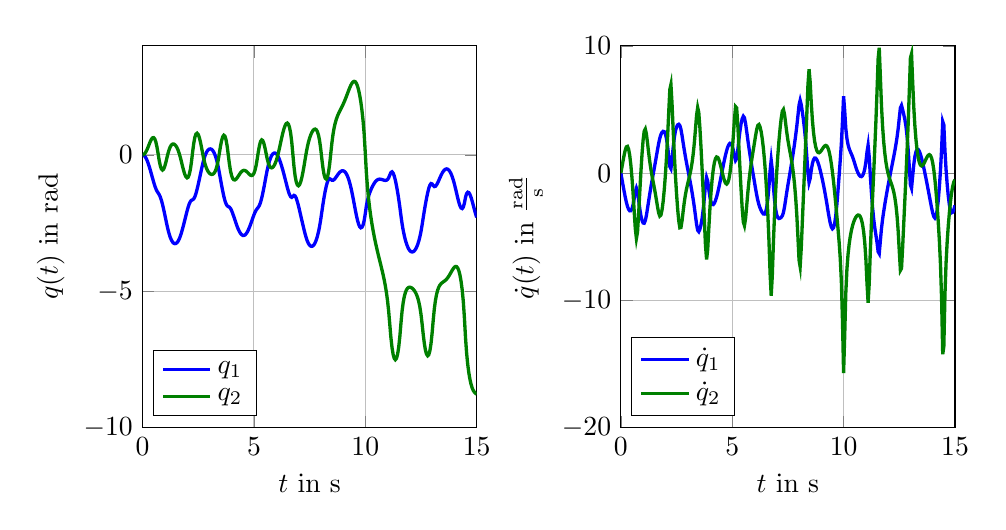
\begin{tikzpicture}

\begin{axis}[%
width=0.35\textwidth,
height=0.4\textwidth,
scale only axis,
xmin=0,
xmax=15,
xlabel={$t$ in $\mathrm{s}$},
xmajorgrids,
ymin=-10,
ymax=4,
ylabel={$q(t)$ in $\mathrm{rad}$},
ymajorgrids,
name=plot1,
legend style={at={(0.03,0.03)},anchor=south west,draw=black,fill=white,legend cell align=left}
]
\addplot [
color=blue,
solid,
line width=1.2pt
]
table[row sep=crcr]{
0 0\\
0.0476350130836029 -0.0111295867215883\\
0.0976350130836029 -0.046733581502918\\
0.147635013083603 -0.106627895971673\\
0.197635013083603 -0.190002627346999\\
0.247635013083603 -0.294935852368999\\
0.297635013083603 -0.418129213257232\\
0.347635013083603 -0.555131240629493\\
0.397635013083603 -0.700757409743321\\
0.447635013083603 -0.849191777595656\\
0.497635013083603 -0.993713457285887\\
0.547635013083603 -1.12651358589171\\
0.597635013083603 -1.23933508385054\\
0.647635013083603 -1.32623526548114\\
0.697635013083603 -1.39090119801248\\
0.747635013083603 -1.45440659632348\\
0.797635013083604 -1.54241516185837\\
0.847635013083604 -1.66486668095307\\
0.897635013083604 -1.81844000881575\\
0.947635013083604 -1.99521747734346\\
0.997635013083604 -2.18661420484584\\
1.0476350130836 -2.38381017714409\\
1.09763501308359 -2.57650046263062\\
1.14763501308359 -2.75322516309959\\
1.19763501308358 -2.90518514724667\\
1.24763501308358 -3.02875724690902\\
1.29763501308357 -3.12395560682695\\
1.34763501308357 -3.19211780362559\\
1.39763501308356 -3.2346657520641\\
1.44763501308355 -3.25263022994329\\
1.49763501308355 -3.24648154969522\\
1.54763501308354 -3.21609958649117\\
1.59763501308354 -3.1609105095684\\
1.64763501308353 -3.08036151509964\\
1.69763501308353 -2.97493177649376\\
1.74763501308352 -2.84733728641912\\
1.79763501308352 -2.7025776044594\\
1.84763501308351 -2.54634391674515\\
1.8976350130835 -2.38378562534094\\
1.9476350130835 -2.21995017368062\\
1.99763501308349 -2.06103212803216\\
2.04763501308349 -1.91532863243021\\
2.09763501308348 -1.79331487575396\\
2.14763501308348 -1.70633118737458\\
2.19763501308347 -1.66140495965131\\
2.24763501308347 -1.64421812617903\\
2.29763501308346 -1.61090460099397\\
2.34763501308346 -1.53346177983173\\
2.39763501308345 -1.41324038290163\\
2.44763501308344 -1.26084755752348\\
2.49763501308344 -1.0872902735027\\
2.54763501308343 -0.901540582843421\\
2.59763501308343 -0.710391054384901\\
2.64763501308342 -0.520259806544859\\
2.69763501308342 -0.339967811776806\\
2.74763501308341 -0.180131306652856\\
2.79763501308341 -0.0476813290821995\\
2.8476350130834 0.0562061158113014\\
2.8976350130834 0.133212817538243\\
2.94763501308339 0.18537851953817\\
2.99763501308338 0.214198348878246\\
3.04763501308338 0.22043983086403\\
3.09763501308337 0.204157838509609\\
3.14763501308337 0.164746572214833\\
3.19763501308336 0.100983378325713\\
3.24763501308336 0.0110393862735527\\
3.29763501308335 -0.107543065820855\\
3.34763501308335 -0.257710599398091\\
3.39763501308334 -0.441557729764207\\
3.44763501308333 -0.655377863007923\\
3.49763501308333 -0.884307810441448\\
3.54763501308332 -1.11035197264225\\
3.59763501308332 -1.32241053270853\\
3.64763501308331 -1.51288968869628\\
3.69763501308331 -1.6730755724129\\
3.7476350130833 -1.79289455113107\\
3.7976350130833 -1.8644872302509\\
3.84763501308329 -1.89356939394271\\
3.89763501308328 -1.91423109629131\\
3.94763501308328 -1.96152949339668\\
3.99763501308327 -2.04156288783941\\
4.04763501308329 -2.1461597333255\\
4.09763501308331 -2.26500371221558\\
4.14763501308332 -2.38886559634459\\
4.19763501308334 -2.5103155908522\\
4.24763501308336 -2.62367280977523\\
4.29763501308337 -2.72464872928337\\
4.34763501308339 -2.80995176784079\\
4.39763501308341 -2.87701346671007\\
4.44763501308342 -2.92387546389835\\
4.49763501308344 -2.94918552044722\\
4.54763501308346 -2.95222678197806\\
4.59763501308347 -2.93293924512111\\
4.64763501308349 -2.89193400505783\\
4.69763501308351 -2.83050949678876\\
4.74763501308352 -2.75066946406644\\
4.79763501308354 -2.65515183120775\\
4.84763501308356 -2.54750518179088\\
4.89763501308357 -2.4322491487051\\
4.94763501308359 -2.3150886249058\\
4.99763501308361 -2.20302450796334\\
5.04763501308362 -2.10400632104424\\
5.09763501308364 -2.02525286857519\\
5.14763501308366 -1.9678859390806\\
5.19763501308367 -1.91700084357696\\
5.24763501308369 -1.84485281840046\\
5.29763501308371 -1.73448488522465\\
5.34763501308372 -1.58530229985118\\
5.39763501308374 -1.40393765692658\\
5.44763501308376 -1.19873188520653\\
5.49763501308377 -0.97892618023213\\
5.54763501308379 -0.757159787572796\\
5.59763501308381 -0.549857383164472\\
5.64763501308382 -0.369959245280136\\
5.69763501308384 -0.222213507078443\\
5.74763501308386 -0.106402572622888\\
5.79763501308387 -0.0208756196002728\\
5.84763501308389 0.0360723632913812\\
5.89763501308391 0.0657951865464525\\
5.94763501308392 0.0691462300668531\\
5.99763501308394 0.0464645970219046\\
6.04763501308396 -0.00215397804579029\\
6.09763501308397 -0.0760702328845227\\
6.14763501308399 -0.173010446183123\\
6.19763501308401 -0.288924485123464\\
6.24763501308402 -0.419494196636791\\
6.29763501308404 -0.56153125039157\\
6.34763501308406 -0.712822020904061\\
6.39763501308407 -0.871000344336777\\
6.44763501308409 -1.03224065731771\\
6.49763501308411 -1.19012144979449\\
6.54763501308412 -1.33498386378286\\
6.59763501308414 -1.45411616241728\\
6.64763501308416 -1.53267431542936\\
6.69763501308417 -1.55552339288765\\
6.74763501308419 -1.52081324457914\\
6.79763501308421 -1.48342387000734\\
6.84763501308422 -1.50380160574636\\
6.89763501308424 -1.5836883010562\\
6.94763501308426 -1.7082189330501\\
6.99763501308427 -1.86223943397503\\
7.04763501308429 -2.03269417670754\\
7.09763501308431 -2.20988041176244\\
7.14763501308432 -2.38780444382173\\
7.19763501308434 -2.56335865322778\\
7.24763501308436 -2.7343305516729\\
7.29763501308438 -2.89624112832378\\
7.34763501308439 -3.04043963664677\\
7.39763501308441 -3.15850319673069\\
7.44763501308443 -3.24752508881369\\
7.49763501308444 -3.30847244557595\\
7.54763501308446 -3.34288328602171\\
7.59763501308448 -3.35154918149281\\
7.64763501308449 -3.33436997076881\\
7.69763501308451 -3.29054955739165\\
7.74763501308453 -3.21884541415798\\
7.79763501308454 -3.11774648290677\\
7.84763501308456 -2.98543118399392\\
7.89763501308458 -2.81931309775643\\
7.94763501308459 -2.61524135670404\\
7.99763501308461 -2.36879422883988\\
8.04763501308458 -2.08885977511029\\
8.09763501308456 -1.80991096573016\\
8.14763501308453 -1.55592391208288\\
8.1976350130845 -1.33197157546657\\
8.24763501308447 -1.14268487685198\\
8.29763501308445 -0.996517427535976\\
8.34763501308442 -0.903582661791184\\
8.39763501308439 -0.871819999041507\\
8.44763501308436 -0.893886877581692\\
8.49763501308433 -0.926076512044332\\
8.54763501308431 -0.930098020313983\\
8.59763501308428 -0.904383556658166\\
8.64763501308425 -0.858499822643164\\
8.69763501308422 -0.801883719217685\\
8.7476350130842 -0.742431287057954\\
8.79763501308417 -0.686503161302997\\
8.84763501308414 -0.6390695782039\\
8.89763501308411 -0.603908641113808\\
8.94763501308408 -0.583848563235685\\
8.99763501308406 -0.581031120887178\\
9.04763501308403 -0.597173951721934\\
9.097635013084 -0.633812439576366\\
9.14763501308397 -0.692493559857392\\
9.19763501308395 -0.774867501072409\\
9.24763501308392 -0.882581631022985\\
9.29763501308389 -1.01685704518243\\
9.34763501308386 -1.1777013129342\\
9.39763501308384 -1.36295347878463\\
9.44763501308381 -1.56762672713033\\
9.49763501308378 -1.78391603605066\\
9.54763501308375 -2.00168730266873\\
9.59763501308372 -2.20890815633987\\
9.6476350130837 -2.39197818604649\\
9.69763501308367 -2.53690160766309\\
9.74763501308364 -2.63201014589613\\
9.79763501308361 -2.67051797246802\\
9.84763501308359 -2.64987374705459\\
9.89763501308356 -2.56710946872158\\
9.94763501308353 -2.4103152893093\\
9.9976350130835 -2.15361037593246\\
10.0476350130835 -1.8690050737192\\
10.0976350130834 -1.66275975785292\\
10.1476350130834 -1.50949407851576\\
10.1976350130834 -1.38665968761479\\
10.2476350130834 -1.28309039638151\\
10.2976350130833 -1.19276009714099\\
10.3476350130833 -1.11274773264946\\
10.3976350130833 -1.0427586868235\\
10.4476350130833 -0.984423535187636\\
10.4976350130832 -0.939674894554359\\
10.5476350130832 -0.909251341745415\\
10.5976350130832 -0.892401533993082\\
10.6476350130831 -0.887343572436055\\
10.6976350130831 -0.891667175013017\\
10.7476350130831 -0.902448981962475\\
10.7976350130831 -0.916183676307717\\
10.847635013083 -0.928633960743044\\
10.897635013083 -0.934609747561783\\
10.947635013083 -0.927576382420887\\
10.9976350130829 -0.89889483026764\\
11.0476350130829 -0.837172652404184\\
11.0976350130829 -0.737512314074784\\
11.1476350130829 -0.644855060063897\\
11.1976350130828 -0.618288298414394\\
11.2476350130828 -0.663119715170224\\
11.2976350130828 -0.769754262019858\\
11.3476350130828 -0.927552712411932\\
11.3976350130827 -1.12539432791012\\
11.4476350130827 -1.35419500809315\\
11.4976350130827 -1.6110081484857\\
11.5476350130826 -1.90102864424768\\
11.5976350130826 -2.21897553591368\\
11.6476350130826 -2.51223603365546\\
11.6976350130826 -2.75333179551537\\
11.7476350130825 -2.95230843408319\\
11.7976350130825 -3.11812562554022\\
11.8476350130825 -3.25506494577486\\
11.8976350130825 -3.36511685863592\\
11.9476350130824 -3.4494629474695\\
11.9976350130824 -3.50911125575735\\
12.0476350130824 -3.54505001398046\\
12.0976350130823 -3.558174548303\\
12.1476350130823 -3.549145002316\\
12.1976350130823 -3.51825473355298\\
12.2476350130823 -3.46533037749737\\
12.2976350130822 -3.38963914275366\\
12.3476350130822 -3.28973516683175\\
12.3976350130822 -3.16312534617212\\
12.4476350130821 -3.00561666070329\\
12.4976350130821 -2.81069727673509\\
12.5476350130821 -2.57333440035316\\
12.5976350130821 -2.30882209565063\\
12.647635013082 -2.05028559438911\\
12.697635013082 -1.81018053636535\\
12.747635013082 -1.58917561211665\\
12.797635013082 -1.39143438086834\\
12.8476350130819 -1.22671259131898\\
12.8976350130819 -1.1082532198481\\
12.9476350130819 -1.05013458090206\\
12.9976350130818 -1.0625815249058\\
13.0476350130818 -1.1229742759404\\
13.0976350130818 -1.1605251706129\\
13.1476350130818 -1.14898285892074\\
13.1976350130817 -1.0988159387753\\
13.2476350130817 -1.02331438732618\\
13.2976350130817 -0.933980689093992\\
13.3476350130816 -0.840466301609055\\
13.3976350130816 -0.750543959895593\\
13.4476350130816 -0.670148421064817\\
13.4976350130816 -0.603590804100589\\
13.5476350130815 -0.553884400205529\\
13.5976350130815 -0.523084898665756\\
13.6476350130815 -0.512586883025375\\
13.6976350130815 -0.523361374055542\\
13.7476350130814 -0.556137357437635\\
13.7976350130814 -0.61152242589774\\
13.8476350130814 -0.690031883370528\\
13.8976350130813 -0.791961732349384\\
13.9476350130813 -0.91701511336243\\
13.9976350130813 -1.06360727647641\\
14.0476350130813 -1.22787767606722\\
14.0976350130812 -1.40264588339841\\
14.1476350130812 -1.57679722411936\\
14.1976350130812 -1.73573548767196\\
14.2476350130811 -1.86330103363371\\
14.2976350130811 -1.9444497603863\\
14.3476350130811 -1.96633938885609\\
14.3976350130811 -1.91477138820688\\
14.447635013081 -1.76646661753094\\
14.497635013081 -1.55171885071406\\
14.547635013081 -1.41507361645506\\
14.597635013081 -1.36627797690494\\
14.6476350130809 -1.38276181545868\\
14.6976350130809 -1.45136526853282\\
14.7476350130809 -1.56073619105731\\
14.7976350130808 -1.69830880941777\\
14.8476350130808 -1.8508682103121\\
14.8976350130808 -2.00635291439859\\
14.9476350130808 -2.15517479940335\\
14.9976350130807 -2.29054422108367\\
};
\addlegendentry{$q_1$};

\addplot [
color=green!50!black,
solid,
line width=1.2pt
]
table[row sep=crcr]{
0 0\\
0.0476350130836029 0.0111290353005154\\
0.0976350130836029 0.0466927772613761\\
0.147635013083603 0.106144364610985\\
0.197635013083603 0.187283243089501\\
0.247635013083603 0.284881279600825\\
0.297635013083603 0.389974704344784\\
0.347635013083603 0.490625455025393\\
0.397635013083603 0.573605013029508\\
0.447635013083603 0.625715636397938\\
0.497635013083603 0.634282661794095\\
0.547635013083603 0.587304467883279\\
0.597635013083603 0.474219254530361\\
0.647635013083603 0.289877234063767\\
0.697635013083603 0.048109928472791\\
0.747635013083603 -0.201590329607086\\
0.797635013083604 -0.399749406064062\\
0.847635013083604 -0.518492722160161\\
0.897635013083604 -0.555415941313562\\
0.947635013083604 -0.517401799797556\\
0.997635013083604 -0.415638839730225\\
1.0476350130836 -0.266689282077423\\
1.09763501308359 -0.094998464739316\\
1.14763501308359 0.0701491681884247\\
1.19763501308358 0.206241385708753\\
1.24763501308358 0.304641366266915\\
1.29763501308357 0.366501989295799\\
1.34763501308357 0.396421475045716\\
1.39763501308356 0.398939466460642\\
1.44763501308355 0.377192524678943\\
1.49763501308355 0.332508251497372\\
1.54763501308354 0.264431963791081\\
1.59763501308354 0.171210114613357\\
1.64763501308353 0.0511618069263267\\
1.69763501308353 -0.0945391717913296\\
1.74763501308352 -0.258527336387989\\
1.79763501308352 -0.426861229202044\\
1.84763501308351 -0.583147034944204\\
1.8976350130835 -0.712543219482007\\
1.9476350130835 -0.802329202684032\\
1.99763501308349 -0.840731708347895\\
2.04763501308349 -0.815904706931043\\
2.09763501308348 -0.715328324591184\\
2.14763501308348 -0.525904822242005\\
2.19763501308347 -0.240685878823509\\
2.24763501308347 0.106788725167448\\
2.29763501308346 0.421608169893294\\
2.34763501308346 0.641812593618658\\
2.39763501308345 0.763254389376223\\
2.44763501308344 0.796527283656376\\
2.49763501308344 0.752800211854154\\
2.54763501308343 0.642841474875024\\
2.59763501308343 0.478352424737698\\
2.64763501308342 0.275342827779717\\
2.69763501308342 0.0584588363317037\\
2.74763501308341 -0.143144338689878\\
2.79763501308341 -0.3108296600652\\
2.8476350130834 -0.441648353948876\\
2.8976350130834 -0.540566091052193\\
2.94763501308339 -0.613693559101387\\
2.99763501308338 -0.665698886043481\\
3.04763501308338 -0.69917403339612\\
3.09763501308337 -0.714557861376675\\
3.14763501308337 -0.710147131235002\\
3.19763501308336 -0.682068265531465\\
3.24763501308336 -0.624196076722496\\
3.29763501308335 -0.528141160778214\\
3.34763501308335 -0.383985569367761\\
3.39763501308334 -0.184543377437384\\
3.44763501308333 0.0609980834091148\\
3.49763501308333 0.313067063838126\\
3.54763501308332 0.523284077365985\\
3.59763501308332 0.663479318567943\\
3.64763501308331 0.720998729227797\\
3.69763501308331 0.687843678089093\\
3.7476350130833 0.556708433985751\\
3.7976350130833 0.323102808084402\\
3.84763501308329 0.00544538183941298\\
3.89763501308328 -0.321419873862096\\
3.94763501308328 -0.581418910094529\\
3.99763501308327 -0.758710038331553\\
4.04763501308329 -0.864333092667897\\
4.09763501308331 -0.91244135401875\\
4.14763501308332 -0.916195907360737\\
4.19763501308334 -0.887644500512129\\
4.24763501308336 -0.837838442600227\\
4.29763501308337 -0.776827957960006\\
4.34763501308339 -0.713561655955735\\
4.39763501308341 -0.655689773018087\\
4.44763501308342 -0.609294578411354\\
4.49763501308344 -0.578634407641521\\
4.54763501308346 -0.565988795290931\\
4.59763501308347 -0.571611189738999\\
4.64763501308349 -0.593730094867231\\
4.69763501308351 -0.628567286091401\\
4.74763501308352 -0.670413164095296\\
4.79763501308354 -0.711810338054072\\
4.84763501308356 -0.743829810119223\\
4.89763501308357 -0.756365680407368\\
4.94763501308359 -0.738392805056177\\
4.99763501308361 -0.678221950279202\\
5.04763501308362 -0.56405664690557\\
5.09763501308364 -0.38638011378851\\
5.14763501308366 -0.147675264288131\\
5.19763501308367 0.116745890341285\\
5.24763501308369 0.344051511078148\\
5.29763501308371 0.492631966584325\\
5.34763501308372 0.552106232156962\\
5.39763501308374 0.525053379679121\\
5.44763501308376 0.419366127787755\\
5.49763501308377 0.250292967393106\\
5.54763501308379 0.0472123904130664\\
5.59763501308381 -0.148004986996979\\
5.64763501308382 -0.302480917725099\\
5.69763501308384 -0.405614252486312\\
5.74763501308386 -0.460553903534244\\
5.79763501308387 -0.474230288089686\\
5.84763501308389 -0.453081595880896\\
5.89763501308391 -0.401738748070293\\
5.94763501308392 -0.322722355826607\\
5.99763501308394 -0.216654737807386\\
6.04763501308396 -0.0832372433604835\\
6.09763501308397 0.076461289905424\\
6.14763501308399 0.256888527135065\\
6.19763501308401 0.447157146293788\\
6.24763501308402 0.634398333466656\\
6.29763501308404 0.807316428349386\\
6.34763501308406 0.956547943085228\\
6.39763501308407 1.07328474397043\\
6.44763501308409 1.14810695075034\\
6.49763501308411 1.17052932565354\\
6.54763501308412 1.12896926864199\\
6.59763501308414 1.01036099339215\\
6.64763501308416 0.798281723014122\\
6.69763501308417 0.470640902656863\\
6.74763501308419 0.0235481592141486\\
6.79763501308421 -0.430527098371278\\
6.84763501308422 -0.767136683872829\\
6.89763501308424 -0.982915202888949\\
6.94763501308426 -1.09902731267667\\
6.99763501308427 -1.13118955843117\\
7.04763501308429 -1.09157913534214\\
7.09763501308431 -0.990764721089398\\
7.14763501308432 -0.838035381267058\\
7.19763501308434 -0.64171552121663\\
7.24763501308436 -0.411296276378141\\
7.29763501308438 -0.16262751749269\\
7.34763501308439 0.0793522425821875\\
7.39763501308441 0.292302388651808\\
7.44763501308443 0.46915191883456\\
7.49763501308444 0.613327806584419\\
7.54763501308446 0.730038760504221\\
7.59763501308448 0.822596153779932\\
7.64763501308449 0.89165673555315\\
7.69763501308451 0.935253107267892\\
7.74763501308453 0.948900376807006\\
7.79763501308454 0.925590779527482\\
7.84763501308456 0.855571634908067\\
7.89763501308458 0.725789833947169\\
7.94763501308459 0.519512366336344\\
7.99763501308461 0.222319693451057\\
8.04763501308458 -0.141144342416388\\
8.09763501308456 -0.477081412401657\\
8.14763501308453 -0.718629643141\\
8.1976350130845 -0.854809696104723\\
8.24763501308447 -0.887257660658783\\
8.29763501308445 -0.816180620702212\\
8.34763501308442 -0.638247610519636\\
8.39763501308439 -0.347703797111591\\
8.44763501308436 0.0382800303735077\\
8.49763501308433 0.428531460428678\\
8.54763501308431 0.744075751270087\\
8.59763501308428 0.983649946864985\\
8.64763501308425 1.16602813156601\\
8.69763501308422 1.307401116043\\
8.7476350130842 1.42031244167471\\
8.79763501308417 1.51475447561056\\
8.84763501308414 1.59881231461944\\
8.89763501308411 1.6789270103559\\
8.94763501308408 1.75999153000148\\
8.99763501308406 1.84539758727308\\
9.04763501308403 1.9370777008484\\
9.097635013084 2.03554545809622\\
9.14763501308397 2.13991989967415\\
9.19763501308395 2.2479265573764\\
9.24763501308392 2.35590222276528\\
9.29763501308389 2.45888623299493\\
9.34763501308386 2.55091066106668\\
9.39763501308384 2.62551645922952\\
9.44763501308381 2.67631418715543\\
9.49763501308378 2.69730377240632\\
9.54763501308375 2.6829098052712\\
9.59763501308372 2.62806738390746\\
9.6476350130837 2.52869220480235\\
9.69763501308367 2.38227383336446\\
9.74763501308364 2.18759131179237\\
9.79763501308361 1.94265279250219\\
9.84763501308359 1.64080919930016\\
9.89763501308356 1.26427499974639\\
9.94763501308353 0.769877075593437\\
9.9976350130835 0.0792887480124395\\
10.0476350130835 -0.657123682131159\\
10.0976350130834 -1.20267741600075\\
10.1476350130834 -1.62197607272577\\
10.1976350130834 -1.96821500759315\\
10.2476350130834 -2.26648385785223\\
10.2976350130833 -2.53006245044988\\
10.3476350130833 -2.76699300464937\\
10.3976350130833 -2.98295063236651\\
10.4476350130833 -3.18248924630044\\
10.4976350130832 -3.36933464989203\\
10.5476350130832 -3.54646671305525\\
10.5976350130832 -3.71649956310009\\
10.6476350130831 -3.88220470230048\\
10.6976350130831 -4.04691130928994\\
10.7476350130831 -4.21476664988776\\
10.7976350130831 -4.39096413465951\\
10.847635013083 -4.58207024114201\\
10.897635013083 -4.79663925922611\\
10.947635013083 -5.04646988868766\\
10.9976350130829 -5.3491050862466\\
11.0476350130829 -5.73087416047076\\
11.0976350130829 -6.20864410380727\\
11.1476350130829 -6.69210751222903\\
11.1976350130828 -7.06101762772697\\
11.2476350130828 -7.31093242075349\\
11.2976350130828 -7.45796475980603\\
11.3476350130828 -7.50796592095666\\
11.3976350130827 -7.46048673548723\\
11.4476350130827 -7.31165276326035\\
11.4976350130827 -7.05260104652025\\
11.5476350130826 -6.66838431844865\\
11.5976350130826 -6.18260037102771\\
11.6476350130826 -5.74043413498406\\
11.6976350130826 -5.41970863674294\\
11.7476350130825 -5.19682193452292\\
11.7976350130825 -5.04470583720227\\
11.8476350130825 -4.94515387321255\\
11.8976350130825 -4.88533491153285\\
11.9476350130824 -4.85562520942457\\
11.9976350130824 -4.84871831372101\\
12.0476350130824 -4.85929792584064\\
12.0976350130823 -4.88392410736735\\
12.1476350130823 -4.92100170666743\\
12.1976350130823 -4.97079786029772\\
12.2476350130823 -5.03551807762172\\
12.2976350130822 -5.11947991162285\\
12.3476350130822 -5.22946760737475\\
12.3976350130822 -5.37542320916727\\
12.4476350130821 -5.571616956854\\
12.4976350130821 -5.83714942472429\\
12.5476350130821 -6.18468870225937\\
12.5976350130821 -6.57186930274052\\
12.647635013082 -6.90780181132663\\
12.697635013082 -7.1531755985173\\
12.747635013082 -7.30508244648406\\
12.797635013082 -7.36310562390224\\
12.8476350130819 -7.32392391593578\\
12.8976350130819 -7.18111475749273\\
12.9476350130819 -6.92264034906022\\
12.9976350130818 -6.53322188700855\\
13.0476350130818 -6.05690068846043\\
13.0976350130818 -5.63999619157084\\
13.1476350130818 -5.33273007142483\\
13.1976350130817 -5.11205655806083\\
13.2476350130817 -4.95523986898363\\
13.2976350130817 -4.84594380668328\\
13.3476350130816 -4.77139428234614\\
13.3976350130816 -4.72080477622932\\
13.4476350130816 -4.68486076850967\\
13.4976350130816 -4.65566167768074\\
13.5476350130815 -4.62679878012471\\
13.5976350130815 -4.5934375531332\\
13.6476350130815 -4.55236448548984\\
13.6976350130815 -4.50199484294438\\
13.7476350130814 -4.44235296040355\\
13.7976350130814 -4.37504538568384\\
13.8476350130814 -4.30324842559093\\
13.8976350130813 -4.23171657592024\\
13.9476350130813 -4.16678179390626\\
13.9976350130813 -4.11626635016849\\
14.0476350130813 -4.08920755602256\\
14.0976350130812 -4.09532957887299\\
14.1476350130812 -4.14430460295227\\
14.1976350130812 -4.2450311594864\\
14.2476350130811 -4.40549631164819\\
14.2976350130811 -4.63426546350186\\
14.3476350130811 -4.94518398630211\\
14.3976350130811 -5.36856135967301\\
14.447635013081 -5.96957471981808\\
14.497635013081 -6.70588937499316\\
14.547635013081 -7.27804387690281\\
14.597635013081 -7.68781752827196\\
14.6476350130809 -7.99668261706183\\
14.6976350130809 -8.23341373729022\\
14.7476350130809 -8.41265501367478\\
14.7976350130808 -8.54423394535767\\
14.8476350130808 -8.63694501818859\\
14.8976350130808 -8.69972554331178\\
14.9476350130808 -8.74157749367677\\
14.9976350130807 -8.77109319447075\\
};
\addlegendentry{$q_2$};

\end{axis}

\begin{axis}[%
width=0.35\textwidth,
height=0.4\textwidth,
scale only axis,
xmin=0,
xmax=15,
xlabel={$t$ in $\mathrm{s}$},
xmajorgrids,
ymin=-20,
ymax=10,
ylabel={$\dot{q}(t)$ in $\mathrm{\frac{rad}{s}}$},
ymajorgrids,
at=(plot1.right of south east),
anchor=left of south west,
legend style={at={(0.03,0.03)},anchor=south west,draw=black,fill=white,legend cell align=left}
]
\addplot [
color=blue,
solid,
line width=1.2pt
]
table[row sep=crcr]{
0 0\\
0.0476350130836029 -0.467258965953613\\
0.0976350130836029 -0.95633893529827\\
0.147635013083603 -1.43692449053459\\
0.197635013083603 -1.89176333988979\\
0.247635013083603 -2.29447971379406\\
0.297635013083603 -2.6182439888838\\
0.347635013083603 -2.84451938598925\\
0.397635013083603 -2.96125769822239\\
0.447635013083603 -2.95380839758302\\
0.497635013083603 -2.80086673967472\\
0.547635013083603 -2.48282861596345\\
0.597635013083603 -2.00786071168611\\
0.647635013083603 -1.47628150500675\\
0.697635013083603 -1.18529449851848\\
0.747635013083603 -1.45001386635608\\
0.797635013083604 -2.10068630964409\\
0.847635013083604 -2.7831512173207\\
0.897635013083604 -3.33221008792189\\
0.947635013083604 -3.71018275420462\\
0.997635013083604 -3.91686772008321\\
1.0476350130836 -3.9367117082842\\
1.09763501308359 -3.73106466319443\\
1.14763501308359 -3.30758277688945\\
1.19763501308358 -2.75952068763557\\
1.24763501308358 -2.18424968018483\\
1.29763501308357 -1.62852315293669\\
1.34763501308357 -1.10284058600335\\
1.39763501308356 -0.602563043589553\\
1.44763501308355 -0.117595281517734\\
1.49763501308355 0.363980124764004\\
1.54763501308354 0.853355775416961\\
1.59763501308354 1.35639387052094\\
1.64763501308353 1.86445096563385\\
1.69763501308353 2.3437550999754\\
1.74763501308352 2.74268594731702\\
1.79763501308352 3.02824516347189\\
1.84763501308351 3.20415273221785\\
1.8976350130835 3.28182512267871\\
1.9476350130835 3.25128729120319\\
1.99763501308349 3.07781783578038\\
2.04763501308349 2.71503035830057\\
2.09763501308348 2.12643756455754\\
2.14763501308348 1.32406827752021\\
2.19763501308347 0.511338876158339\\
2.24763501308347 0.348185877398358\\
2.29763501308346 1.07827456112119\\
2.34763501308346 2.00643031455415\\
2.39763501308345 2.76480286213582\\
2.44763501308344 3.2935302713539\\
2.49763501308344 3.61879883746705\\
2.54763501308343 3.78916169825639\\
2.59763501308343 3.83658457218311\\
2.64763501308342 3.73931744313391\\
2.69763501308342 3.43444539874784\\
2.74763501308341 2.93521922940704\\
2.79763501308341 2.36020755832718\\
2.8476350130834 1.8017280642411\\
2.8976350130834 1.2855846944716\\
2.94763501308339 0.806066385348816\\
2.99763501308338 0.349274520808311\\
3.04763501308338 -0.0994511849303295\\
3.09763501308337 -0.553863619082144\\
3.14763501308337 -1.02666700493648\\
3.19763501308336 -1.52994445249498\\
3.24763501308336 -2.07601665370733\\
3.29763501308335 -2.67740950770238\\
3.34763501308335 -3.33786392219729\\
3.39763501308334 -4.00665754611492\\
3.44763501308333 -4.49314884308039\\
3.49763501308333 -4.59947958345935\\
3.54763501308332 -4.40761332015892\\
3.59763501308332 -4.05105948795466\\
3.64763501308331 -3.53904209216873\\
3.69763501308331 -2.83378011601604\\
3.7476350130833 -1.92954207309719\\
3.7976350130833 -0.944623386182345\\
3.84763501308329 -0.343731277026525\\
3.89763501308328 -0.613334497960544\\
3.94763501308328 -1.28976774643015\\
3.99763501308327 -1.88083935930977\\
4.04763501308329 -2.26785501040769\\
4.09763501308331 -2.45495365873031\\
4.14763501308332 -2.47478965573999\\
4.19763501308334 -2.36440561241134\\
4.24763501308336 -2.15572770277276\\
4.29763501308337 -1.87243001838919\\
4.34763501308339 -1.5311646056801\\
4.39763501308341 -1.14477263317295\\
4.44763501308342 -0.725188052292539\\
4.49763501308344 -0.284817937603785\\
4.54763501308346 0.163371613188696\\
4.59763501308347 0.606098527809744\\
4.64763501308349 1.02978874344654\\
4.69763501308351 1.42052007777863\\
4.74763501308352 1.76397796584843\\
4.79763501308354 2.04495313418839\\
4.84763501308356 2.24592599147083\\
4.89763501308357 2.34535128571948\\
4.94763501308359 2.31765077569144\\
4.99763501308361 2.13795807263529\\
5.04763501308362 1.79713622942448\\
5.09763501308364 1.3451779134449\\
5.14763501308366 0.998541196719709\\
5.19763501308367 1.14127897891792\\
5.24763501308369 1.80162355130579\\
5.29763501308371 2.61115724102559\\
5.34763501308372 3.33232484543689\\
5.39763501308374 3.89420087957985\\
5.44763501308376 4.28427574847092\\
5.49763501308377 4.4665476113468\\
5.54763501308379 4.34608609924398\\
5.59763501308381 3.90099996883296\\
5.64763501308382 3.28079745607188\\
5.69763501308384 2.63096308428382\\
5.74763501308386 2.00735554236993\\
5.79763501308387 1.41951137795921\\
5.84763501308389 0.862967193397091\\
5.89763501308391 0.328802701015631\\
5.94763501308392 -0.193706446864131\\
5.99763501308394 -0.713502377612943\\
6.04763501308396 -1.22954469353663\\
6.09763501308397 -1.71964215466868\\
6.14763501308399 -2.14383685577175\\
6.19763501308401 -2.47778003824404\\
6.24763501308402 -2.73448736399122\\
6.29763501308404 -2.94003092009419\\
6.34763501308406 -3.10415950694611\\
6.39763501308407 -3.21061568516314\\
6.44763501308409 -3.21782613294311\\
6.49763501308411 -3.06514550794499\\
6.54763501308412 -2.68663751612767\\
6.59763501308414 -2.0287693117747\\
6.64763501308416 -1.06090523245604\\
6.69763501308417 0.173690211035988\\
6.74763501308419 1.01540709245101\\
6.79763501308421 0.248746564258418\\
6.84763501308422 -1.04643500608747\\
6.89763501308424 -2.09665805032784\\
6.94763501308426 -2.83353029360816\\
6.99763501308427 -3.28330915550825\\
7.04763501308429 -3.50240895149314\\
7.09763501308431 -3.56534382678834\\
7.14763501308432 -3.54190572563321\\
7.19763501308434 -3.47400493659259\\
7.24763501308436 -3.35100230100813\\
7.29763501308438 -3.09481184647263\\
7.34763501308439 -2.64262450799087\\
7.39763501308441 -2.07132860232367\\
7.44763501308443 -1.49399549796207\\
7.49763501308444 -0.949386970800776\\
7.54763501308446 -0.429697026377884\\
7.59763501308448 0.0834705643949696\\
7.64763501308449 0.606439411701224\\
7.69763501308451 1.15058499174873\\
7.74763501308453 1.72261397908036\\
7.79763501308454 2.32727005559966\\
7.84763501308456 2.97363918686926\\
7.89763501308458 3.68486821053564\\
7.94763501308459 4.49652274354815\\
7.99763501308461 5.34255198432683\\
8.04763501308458 5.71767148224964\\
8.09763501308456 5.36176974683015\\
8.14763501308453 4.78841283463119\\
8.1976350130845 4.15488464049012\\
8.24763501308447 3.38748058482732\\
8.29763501308445 2.42447918467582\\
8.34763501308442 1.26336986863776\\
8.39763501308439 0.018393154599876\\
8.44763501308436 -0.735216447970361\\
8.49763501308433 -0.413251604113429\\
8.54763501308431 0.244483549966636\\
8.59763501308428 0.749711020758727\\
8.64763501308425 1.05398392787487\\
8.69763501308422 1.18436758549829\\
8.7476350130842 1.17257595665563\\
8.79763501308417 1.04804809809394\\
8.84763501308414 0.836783559590819\\
8.89763501308411 0.56031544011571\\
8.94763501308408 0.235036668250542\\
8.99763501308406 -0.127982643192796\\
9.04763501308403 -0.522781492709237\\
9.097635013084 -0.947879475124685\\
9.14763501308397 -1.40489488070992\\
9.19763501308395 -1.89569127834149\\
9.24763501308392 -2.41721515087134\\
9.29763501308389 -2.9541704675103\\
9.34763501308386 -3.47263885355852\\
9.39763501308384 -3.920812278745\\
9.44763501308381 -4.23990369491365\\
9.49763501308378 -4.37773648034053\\
9.54763501308375 -4.29295011354049\\
9.59763501308372 -3.95021922069609\\
9.6476350130837 -3.32493282071366\\
9.69763501308367 -2.43206527376706\\
9.74763501308364 -1.34985075585726\\
9.79763501308361 -0.18356554502737\\
9.84763501308359 1.01654246610965\\
9.89763501308356 2.32895940444902\\
9.94763501308353 4.05037530450412\\
9.9976350130835 6.04598797442252\\
10.0476350130835 4.89701217397679\\
10.0976350130834 3.49065075149484\\
10.1476350130834 2.71100753555226\\
10.1976350130834 2.23767341129341\\
10.2476350130834 1.92462836900465\\
10.2976350130833 1.69824550715086\\
10.3476350130833 1.50304580680023\\
10.3976350130833 1.29046885006659\\
10.4476350130833 1.03592644346312\\
10.4976350130832 0.751498176940288\\
10.5476350130832 0.468147804140107\\
10.5976350130832 0.211924587586959\\
10.6476350130831 -0.00154097547153587\\
10.6976350130831 -0.161686840492464\\
10.7476350130831 -0.257951600331906\\
10.7976350130831 -0.277380907306778\\
10.847635013083 -0.203449857036187\\
10.897635013083 -0.0140457010322801\\
10.947635013083 0.323771127891849\\
10.9976350130829 0.86244042654745\\
11.0476350130829 1.64063076729597\\
11.0976350130829 2.19196486772385\\
11.1476350130829 1.27976469634431\\
11.1976350130828 -0.210863039518596\\
11.2476350130828 -1.54876842058268\\
11.2976350130828 -2.68132926941776\\
11.3476350130828 -3.59261840886557\\
11.3976350130827 -4.28927089426302\\
11.4476350130827 -4.85177640463777\\
11.4976350130827 -5.44114810746049\\
11.5476350130826 -6.16955828662017\\
11.5976350130826 -6.32241777508541\\
11.6476350130826 -5.32919360918095\\
11.6976350130826 -4.3608412549655\\
11.7476350130825 -3.62760493418293\\
11.7976350130825 -3.01846316604245\\
11.8476350130825 -2.46527153247799\\
11.8976350130825 -1.94054949893995\\
11.9476350130824 -1.436614898636\\
11.9976350130824 -0.952643263568219\\
12.0476350130824 -0.487942552437538\\
12.0976350130823 -0.0392840492890085\\
12.1476350130823 0.399455895826796\\
12.1976350130823 0.836704989569892\\
12.2476350130823 1.28266634806895\\
12.2976350130822 1.74969943539538\\
12.3476350130822 2.25455243902747\\
12.3976350130822 2.82349615014923\\
12.4476350130821 3.49902439969306\\
12.4976350130821 4.3214733343949\\
12.5476350130821 5.12722059704912\\
12.5976350130821 5.31825959776912\\
12.647635013082 4.99152307700298\\
12.697635013082 4.61512783964059\\
12.747635013082 4.21143424636827\\
12.797635013082 3.66486118348468\\
12.8476350130819 2.87892233274509\\
12.8976350130819 1.81180154701707\\
12.9476350130819 0.47182713633486\\
12.9976350130818 -0.919918029920146\\
13.0476350130818 -1.1919198060204\\
13.0976350130818 -0.246302412621509\\
13.1476350130818 0.663776282320706\\
13.1976350130817 1.29816081973062\\
13.2476350130817 1.68360281840455\\
13.2976350130817 1.85754865602396\\
13.3476350130816 1.85712682298038\\
13.3976350130816 1.72006005698334\\
13.4476350130816 1.4815048734839\\
13.4976350130816 1.17087163814727\\
13.5476350130815 0.810631541600044\\
13.5976350130815 0.41677873351439\\
13.6476350130815 -3.42445313233648e-05\\
13.6976350130815 -0.433333746524181\\
13.7476350130814 -0.879718084544449\\
13.7976350130814 -1.33744007020379\\
13.8476350130814 -1.80404512375975\\
13.8976350130813 -2.27239136398777\\
13.9476350130813 -2.72480152549667\\
13.9976350130813 -3.12638834178109\\
14.0476350130813 -3.42073046219439\\
14.0976350130812 -3.53282469577424\\
14.1476350130812 -3.38390995745853\\
14.1976350130812 -2.91873914336364\\
14.2476350130811 -2.13321677074015\\
14.2976350130811 -1.07098561168278\\
14.3476350130811 0.239213905804041\\
14.3976350130811 1.90394355210032\\
14.447635013081 4.0519994870164\\
14.497635013081 3.7868433389032\\
14.547635013081 1.75648480960334\\
14.597635013081 0.269633948280154\\
14.6476350130809 -0.888050309605726\\
14.6976350130809 -1.81913442866951\\
14.7476350130809 -2.51351251294231\\
14.7976350130808 -2.94465204597257\\
14.8476350130808 -3.11705994189854\\
14.8976350130808 -3.07028095802705\\
14.9476350130808 -2.86010436395882\\
14.9976350130807 -2.54038686727618\\
};
\addlegendentry{$\dot{q}_1$};

\addplot [
color=green!50!black,
solid,
line width=1.2pt
]
table[row sep=crcr]{
0 0\\
0.0476350130836029 0.467189515664757\\
0.0976350130836029 0.953834854131957\\
0.147635013083603 1.41741321921243\\
0.197635013083603 1.81100211600005\\
0.247635013083603 2.06275417407624\\
0.297635013083603 2.10054823131349\\
0.347635013083603 1.88092587928252\\
0.397635013083603 1.39413060716618\\
0.447635013083603 0.648033836691204\\
0.497635013083603 -0.345523066476585\\
0.547635013083603 -1.56979757398976\\
0.597635013083603 -2.97497747912182\\
0.647635013083603 -4.36154450942767\\
0.697635013083603 -5.13483540183815\\
0.747635013083603 -4.63510129555309\\
0.797635013083604 -3.20479039361071\\
0.847635013083604 -1.54270478601511\\
0.897635013083604 0.0415776307920799\\
0.947635013083604 1.44218476963878\\
0.997635013083604 2.57431610366399\\
1.0476350130836 3.30157246886955\\
1.09763501308359 3.46360511999384\\
1.14763501308359 3.06448254368242\\
1.19763501308358 2.3524913920957\\
1.24763501308358 1.58965813458006\\
1.29763501308357 0.901181592789849\\
1.34763501308357 0.311117352191993\\
1.39763501308356 -0.19982848416272\\
1.44763501308355 -0.665631046593222\\
1.49763501308355 -1.12339540176961\\
1.54763501308354 -1.60592268338191\\
1.59763501308354 -2.12949812927517\\
1.64763501308353 -2.66984027579174\\
1.69763501308353 -3.13392926771193\\
1.74763501308352 -3.37741713102867\\
1.79763501308352 -3.29976912065827\\
1.84763501308351 -2.9021502560246\\
1.8976350130835 -2.23178296776612\\
1.9476350130835 -1.32075091933127\\
1.99763501308349 -0.176046858737938\\
2.04763501308349 1.21073977864054\\
2.09763501308348 2.85709840825438\\
2.14763501308348 4.75349187344762\\
2.19763501308347 6.56542377898066\\
2.24763501308347 6.96203050476929\\
2.29763501308346 5.42523051788063\\
2.34763501308346 3.38715449289525\\
2.39763501308345 1.50878220064968\\
2.44763501308344 -0.140652297608493\\
2.49763501308344 -1.57292909265042\\
2.54763501308343 -2.78750187603843\\
2.59763501308343 -3.74065214810252\\
2.64763501308342 -4.29676969569187\\
2.69763501308342 -4.27464453555117\\
2.74763501308341 -3.7256806632617\\
2.79763501308341 -2.97547272894202\\
2.8476350130834 -2.27608779665616\\
2.8976350130834 -1.70171180025055\\
2.94763501308339 -1.23909912912054\\
2.99763501308338 -0.849761918121941\\
3.04763501308338 -0.490698612199812\\
3.09763501308337 -0.118985753464061\\
3.14763501308337 0.308296309210358\\
3.19763501308336 0.835249425093954\\
3.24763501308336 1.50774381947929\\
3.29763501308335 2.3685817393709\\
3.34763501308335 3.42604394050926\\
3.39763501308334 4.52878924504715\\
3.44763501308333 5.15186520781878\\
3.49763501308333 4.75668740312433\\
3.54763501308332 3.56249589687987\\
3.59763501308332 2.00696582452536\\
3.64763501308331 0.2682522255833\\
3.69763501308331 -1.61902334050568\\
3.7476350130833 -3.64652663717728\\
3.7976350130833 -5.6555693961874\\
3.84763501308329 -6.77819024974008\\
3.89763501308328 -6.01417057447385\\
3.94763501308328 -4.35352007274949\\
3.99763501308327 -2.78137523371102\\
4.04763501308329 -1.49140866813905\\
4.09763501308331 -0.476733476074847\\
4.14763501308332 0.286433677374427\\
4.19763501308334 0.818780846045235\\
4.24763501308336 1.13992807953229\\
4.29763501308337 1.27059634192065\\
4.34763501308339 1.2344603226216\\
4.39763501308341 1.06005038305462\\
4.44763501308342 0.78151118142628\\
4.49763501308344 0.43728525525977\\
4.54763501308346 0.0676967303557171\\
4.59763501308347 -0.28668400710263\\
4.64763501308349 -0.585456253383905\\
4.69763501308351 -0.788937346830944\\
4.74763501308352 -0.859943417322546\\
4.79763501308354 -0.766078848985032\\
4.84763501308356 -0.480928811322541\\
4.89763501308357 0.0163201840501101\\
4.94763501308359 0.741694884207053\\
4.99763501308361 1.70502558655573\\
5.04763501308362 2.89597658884269\\
5.09763501308364 4.21131540430026\\
5.14763501308366 5.22128690348572\\
5.19763501308367 5.12097664613444\\
5.24763501308369 3.8325756113452\\
5.29763501308371 2.08391112156969\\
5.34763501308372 0.305743504147727\\
5.39763501308374 -1.36233115592113\\
5.44763501308376 -2.8171190934404\\
5.49763501308377 -3.84869257441007\\
5.54763501308379 -4.12552644622157\\
5.59763501308381 -3.56838558033393\\
5.64763501308382 -2.57979560200379\\
5.69763501308384 -1.5594762358116\\
5.74763501308386 -0.662438162649818\\
5.79763501308387 0.0935677692014538\\
5.84763501308389 0.736860470892015\\
5.89763501308391 1.30850862745245\\
5.94763501308392 1.85036371951171\\
5.99763501308394 2.39409756574776\\
6.04763501308396 2.94025207887206\\
6.09763501308397 3.42964421948464\\
6.14763501308399 3.74974548161946\\
6.19763501308401 3.81671519706449\\
6.24763501308402 3.63529566017624\\
6.29763501308404 3.25077480286808\\
6.34763501308406 2.68952899534173\\
6.39763501308407 1.94867936729604\\
6.44763501308409 1.00923266062505\\
6.49763501308411 -0.150878888393472\\
6.54763501308412 -1.5544915878057\\
6.59763501308414 -3.24325068656035\\
6.64763501308416 -5.31600658744139\\
6.69763501308417 -7.84833742150128\\
6.74763501308419 -9.62831872468898\\
6.79763501308421 -8.05725919014208\\
6.84763501308422 -5.44825823305002\\
6.89763501308424 -3.25719006414604\\
6.94763501308426 -1.43831027679926\\
6.99763501308427 0.111838007160632\\
7.04763501308429 1.43737698609258\\
7.09763501308431 2.56425698357176\\
7.14763501308432 3.51777833703281\\
7.19763501308434 4.30525510598306\\
7.24763501308436 4.86061556409994\\
7.29763501308438 4.99833702626284\\
7.34763501308439 4.60058551482919\\
7.39763501308441 3.89682169897257\\
7.44763501308443 3.19178950265046\\
7.49763501308444 2.59363748460493\\
7.54763501308446 2.08599621124157\\
7.59763501308448 1.61845284902618\\
7.64763501308449 1.13737077875078\\
7.69763501308451 0.591532182953363\\
7.74763501308453 -0.0689341423155768\\
7.79763501308454 -0.895771681965705\\
7.84763501308456 -1.94822499278786\\
7.89763501308458 -3.29963998220786\\
7.94763501308459 -5.01012426384225\\
7.99763501308461 -6.82236260966172\\
8.04763501308458 -7.34594671585975\\
8.09763501308456 -5.86893046400482\\
8.14763501308453 -3.77454290468005\\
8.1976350130845 -1.68091996059072\\
8.24763501308447 0.381936852107026\\
8.29763501308445 2.47186917037269\\
8.34763501308442 4.66991850600623\\
8.39763501308439 6.92562231781099\\
8.44763501308436 8.1675968948627\\
8.49763501308433 7.15522163827347\\
8.54763501308431 5.49167705621631\\
8.59763501308428 4.15841250093876\\
8.64763501308425 3.19043261855162\\
8.69763501308422 2.50588888583962\\
8.7476350130842 2.0436700455091\\
8.79763501308417 1.7608845457241\\
8.84763501308414 1.6228725008148\\
8.89763501308411 1.59801146199219\\
8.94763501308408 1.65586098040858\\
8.99763501308406 1.76680876944737\\
9.04763501308403 1.90209901586768\\
9.097635013084 2.03367545851241\\
9.14763501308397 2.13372310329059\\
9.19763501308395 2.1743084152918\\
9.24763501308392 2.1280886636834\\
9.29763501308389 1.97119733318687\\
9.34763501308386 1.6880454454394\\
9.39763501308384 1.27477796846269\\
9.44763501308381 0.737138752334992\\
9.49763501308378 0.0838528555764519\\
9.54763501308375 -0.676661175929902\\
9.59763501308372 -1.53090332440391\\
9.6476350130837 -2.4524312159843\\
9.69763501308367 -3.40767543767324\\
9.74763501308364 -4.38497346645529\\
9.79763501308361 -5.43278462621982\\
9.84763501308359 -6.69610407715882\\
9.89763501308356 -8.49875739289176\\
9.94763501308353 -11.5871379205057\\
9.9976350130835 -15.7011707546524\\
10.0476350130835 -12.7625748152186\\
10.0976350130834 -9.39786168735173\\
10.1476350130834 -7.54071982780994\\
10.1976350130834 -6.38752059244004\\
10.2476350130834 -5.58558837084597\\
10.2976350130833 -4.98348044202761\\
10.3476350130833 -4.51226190030313\\
10.3976350130833 -4.14116664999974\\
10.4476350130833 -3.85280024267926\\
10.4976350130832 -3.63080643430191\\
10.5476350130832 -3.46300026063608\\
10.5976350130832 -3.3474199106105\\
10.6476350130831 -3.29180199078992\\
10.6976350130831 -3.31021634090511\\
10.7476350130831 -3.4212078206316\\
10.7976350130831 -3.64839049608632\\
10.847635013083 -4.02397978109417\\
10.897635013083 -4.59730820173195\\
10.947635013083 -5.45299013401638\\
10.9976350130829 -6.74139300151788\\
11.0476350130829 -8.62541221393471\\
11.0976350130829 -10.1770567723266\\
11.1476350130829 -8.6785883060942\\
11.1976350130828 -6.11966685935215\\
11.2476350130828 -3.93399466675803\\
11.2976350130828 -1.96465585422176\\
11.3476350130828 -0.0328716631805177\\
11.3976350130827 1.94436242626607\\
11.4476350130827 4.03692021008368\\
11.4976350130827 6.38221464359555\\
11.5476350130826 8.97297223815588\\
11.5976350130826 9.84581513459147\\
11.6476350130826 7.61167379930067\\
11.6976350130826 5.32875073497487\\
11.7476350130825 3.67691774924133\\
11.7976350130825 2.46700418787343\\
11.8476350130825 1.55717214264877\\
11.8976350130825 0.867403139878707\\
11.9476350130824 0.345245776883603\\
11.9976350130824 -0.0512815654805118\\
12.0476350130824 -0.360445805225881\\
12.0976350130823 -0.619278988424817\\
12.1476350130823 -0.864691808025252\\
12.1976350130823 -1.13445182502924\\
12.2476350130823 -1.46863785257739\\
12.2976350130822 -1.91223039226829\\
12.3476350130822 -2.52001465654322\\
12.3976350130822 -3.36530818965997\\
12.4476350130821 -4.54790168071132\\
12.4976350130821 -6.13362647190538\\
12.5476350130821 -7.63946323156122\\
12.5976350130821 -7.48225877993434\\
12.647635013082 -5.84575858453165\\
12.697635013082 -3.96979305839486\\
12.747635013082 -2.10565768230739\\
12.797635013082 -0.204010667571413\\
12.8476350130819 1.79176040569466\\
12.8976350130819 3.95946706066542\\
12.9476350130819 6.44478228897784\\
12.9976350130818 9.04671892887382\\
13.0476350130818 9.36821421393188\\
13.0976350130818 7.19649996335548\\
13.1476350130818 5.19037828411352\\
13.1976350130817 3.71187444005254\\
13.2476350130817 2.61415905419572\\
13.2976350130817 1.79977808100801\\
13.3476350130816 1.2180154288462\\
13.3976350130816 0.836608110345781\\
13.4476350130816 0.627518905767361\\
13.4976350130816 0.561836071210428\\
13.5476350130815 0.608810538221245\\
13.5976350130815 0.736352257727503\\
13.6476350130815 0.911845310049803\\
13.6976350130815 1.10284916302559\\
13.7476350130814 1.27746632571135\\
13.7976350130814 1.40425308949872\\
13.8476350130814 1.45178059294857\\
13.8976350130813 1.38836321242727\\
13.9476350130813 1.18286576009866\\
13.9976350130813 0.807449979686004\\
14.0476350130813 0.242232042815016\\
14.0976350130812 -0.519619388260519\\
14.1476350130812 -1.46914006422388\\
14.1976350130812 -2.58611960146258\\
14.2476350130811 -3.85959357063475\\
14.2976350130811 -5.33396448908236\\
14.3476350130811 -7.19595319594973\\
14.3976350130811 -9.9613033790684\\
14.447635013081 -14.230419906644\\
14.497635013081 -13.6061321539192\\
14.547635013081 -9.54084673988189\\
14.597635013081 -7.05115641754182\\
14.6476350130809 -5.39260680363535\\
14.6976350130809 -4.12268040371818\\
14.7476350130809 -3.0785782786187\\
14.7976350130808 -2.2135611379632\\
14.8476350130808 -1.5247405610005\\
14.8976350130808 -1.01666498678089\\
14.9476350130808 -0.686201948608723\\
14.9976350130807 -0.520351485455087\\
};
\addlegendentry{$\dot{q}_2$};

\end{axis}
\end{tikzpicture}%
	\caption{Verification of the model with \usebox{\modeliii}}
	\label{fig:ch1_model3}
\end{figure}
As the simulation results fit with the expectations, the derived dynamic model can be seen as correct. The next step is to design a controller for the motion of the robot.